\section{Identification and the logic of empirical models}\label{sec:A-identification}

Every empirical claim in this book rests on an argument that the data, together with stated assumptions,
pin down the object of interest. This section makes that argument precise. It defines identification,
shows how simultaneity and selection defeat naive comparisons, and describes the Monte Carlo experiments
that the book uses to study estimators.

\subsection{Models, structures and identification}\label{sec:A-models}

We separate four objects. The \emph{observables} $w$ are the variables in the data, such as prices,
quantities and cost shifters. A \emph{structure} $S$ specifies every primitive of the economic model:
demand and cost functions, the rule that determines conduct, and the joint distribution of the
unobservables. Each structure implies a distribution of the observables, which we write $F_w(\cdot\,; S)$.
A \emph{model} $\mathcal{M}$ is the set of structures that satisfy the maintained assumptions. A
\emph{feature} $\psi = \psi(S)$ is any quantity we want to learn, such as a slope, an elasticity, a markup
or a counterfactual price.

\begin{definition}[Identification]\label{def:A-identification}
Let $\mathcal{M}$ be a model and let $S_0 \in \mathcal{M}$ be the structure that generated the data.
\begin{enumerate}[label=(\roman*)]
\item Two structures $S, S' \in \mathcal{M}$ are \emph{observationally equivalent} if
  $F_w(\cdot\,; S) = F_w(\cdot\,; S')$.
\item The feature $\psi$ is \emph{point identified} at $S_0$ if $\psi(S) = \psi(S_0)$ for every
  $S \in \mathcal{M}$ that is observationally equivalent to $S_0$. It is \emph{identified} in $\mathcal{M}$
  if this holds at every $S_0 \in \mathcal{M}$.
\item The \emph{identified set} of $\psi$ at $S_0$ is
  \begin{equation*}
  \Psi_I(S_0) = \bigl\{\psi(S) : S \in \mathcal{M},\ F_w(\cdot\,; S) = F_w(\cdot\,; S_0)\bigr\}.
  \end{equation*}
  The feature is \emph{partially identified} when $\Psi_I(S_0)$ contains more than one point and is a
  proper subset of the values that $\psi$ can take in $\mathcal{M}$.
\end{enumerate}
\end{definition}

Identification is a property of the model and of the population distribution of the observables. It comes
logically before estimation, which concerns finite samples. If two structures produce the same distribution
of data, no sample of any size can tell them apart. \citet[pp.~2108--2109]{AtheyHaile2002} draw three
lessons that apply throughout the book. First, whether a model is identified is a question distinct from
the choice of approximation used for estimation. Second, when a model is nonparametrically identified, a
parametric specification can serve as a parsimonious approximation instead of a maintained hypothesis.
Third, a failure of identification need not preclude testing. They show, for instance, that private values
can be tested against common values in auctions even when neither model is identified
(\cref{ch:auction-empirics}).

\casehead{Moment conditions and local identification}
Much of the book defines the parameter through moment conditions. Let $g(w; \theta)$ be an $L \times 1$
vector of functions, and suppose the true value solves
\begin{equation}\label{eq:A-moment-id}
m(\theta_0) \equiv \E[g(w_i; \theta_0)] = 0 .
\end{equation}
The parameter is identified by \eqref{eq:A-moment-id} if $\theta_0$ is the only zero of $m(\cdot)$ in
$\Theta$. It is \emph{locally identified} if $\theta_0$ is the only zero in some neighborhood of $\theta_0$.
Local identification has a simple sufficient condition.

\begin{proposition}[Local identification from a rank condition]\label{prop:A-local-id}
Suppose $m(\theta_0) = 0$, $m$ is differentiable at $\theta_0$, and the $L \times K$ Jacobian
$G = \frac{\partial m(\theta_0)}{\partial\theta^\top}$ has full column rank $K$. Then there is a neighborhood
$\mathcal{N}$ of $\theta_0$ such that $m(\theta) \neq 0$ for every $\theta \in \mathcal{N}$ with
$\theta \neq \theta_0$.
\end{proposition}

\begin{proof}
Let $c^2$ be the smallest eigenvalue of $G^\top G$. It is positive because $G$ has full column rank. For any
$h \in \R^K$,
\begin{equation*}
\lVert Gh\rVert^2 = h^\top G^\top G h \ge c^2\lVert h\rVert^2 .
\end{equation*}
Differentiability at $\theta_0$ gives $m(\theta) = G(\theta - \theta_0) + r(\theta)$ with
$\frac{\lVert r(\theta)\rVert}{\lVert\theta - \theta_0\rVert} \to 0$ as $\theta \to \theta_0$. Choose a ball
$\mathcal{N}$ around $\theta_0$ on which $\lVert r(\theta)\rVert \le \frac{c}{2}\lVert\theta - \theta_0\rVert$.
For $\theta \in \mathcal{N}$ with $\theta \neq \theta_0$,
\begin{equation*}
\lVert m(\theta)\rVert \ge \lVert G(\theta - \theta_0)\rVert - \lVert r(\theta)\rVert
\ge c\lVert\theta - \theta_0\rVert - \frac{c}{2}\lVert\theta - \theta_0\rVert > 0 .
\qedhere
\end{equation*}
\end{proof}

\citet{Rothenberg1971} gives the likelihood version of this result. When $\theta_0$ is a regular point of the
information matrix, $\theta_0$ is locally identified if and only if the information matrix is nonsingular.
In linear models, $m(\theta) = \E[z_i y_i] - \E[z_i x_i^\top]\theta$ has a constant Jacobian, so the rank
condition delivers global identification. Nonlinear models need a global argument as well, such as the
invertibility of market shares in the demand chapters (\cref{sec:07-invertibility,ch:blp}). A rank failure
means that some direction in the parameter space leaves the moments unchanged to first order. The conduct parameter of
\cref{sec:A-simeq} gives an example.

\casehead{Normalizations}
Some parameters are unidentified because the model is invariant to a transformation of the structure. A
\emph{normalization} resolves the invariance by picking one structure from each class of observationally
equivalent structures. In discrete choice, adding a constant to every utility, or multiplying every utility
by a positive number, leaves choices unchanged (\cref{prop:06-normalization}). The level of utility is
therefore fixed by setting the outside good's mean utility to zero, and its scale by fixing the variance of
the idiosyncratic shock.

The vertical model gives a sharper example. Consumer $i$ obtains utility $u_{ij} = \delta_j - \nu_i p_j$
from product $j$, with quality $\delta_j = x_{jt}\beta + \xi_{jt}$. The price sensitivity $\nu_i$ is
exponential with rate $\lambda$, so $\E[\nu_i] = \frac{1}{\lambda}$. Fix $c > 0$ and multiply every utility
by $c$:
\begin{equation*}
c\,u_{ij} = c\,\delta_j - (c\,\nu_i)\,p_j .
\end{equation*}
Choices do not change. The rescaled sensitivity satisfies
$\Pr(c\,\nu_i \le v) = \Pr\bigl(\nu_i \le \frac{v}{c}\bigr) = 1 - e^{-\frac{\lambda}{c}v}$, so it is
exponential with rate $\frac{\lambda}{c}$. The structures $(\beta, \xi, \lambda)$ and
$(c\beta, c\xi, \frac{\lambda}{c})$ therefore imply the same market shares for every $c > 0$. Only the
products $\lambda\beta$ and $\lambda\xi$ are identified. The normalization $\lambda = 1$ measures quality in
units of willingness to pay (\cref{sec:06-vinversion,app:problems}).

\casehead{Identification needs restrictions}
A model that admits every structure explains every data set, and then no feature is identified. The
conduct parameter of \cref{ch:conduct} shows this starkly. Write the pricing relation with conduct free for
every observation:
\begin{equation}\label{eq:A-free-conduct}
P_{it} = mc_{it} + \theta_{it}\,\frac{Q_{it}}{\left\lvert\frac{\partial Q_{it}}{\partial P_{it}}\right\rvert} .
\end{equation}
Here $\theta_{it}$ is the conduct parameter. Take any observed $(P_{it}, Q_{it})$, any demand slope and any
marginal cost function $mc_{it} = c(Q_{it}; \gamma)$. Setting
\begin{equation*}
\theta_{it} = \frac{(P_{it} - mc_{it})\left\lvert\frac{\partial Q_{it}}{\partial P_{it}}\right\rvert}{Q_{it}}
\end{equation*}
reproduces the data exactly, without an error term. Every cost function is then observationally
equivalent to every other one. The model acquires content only after we restrict $\theta_{it}$. It can be
constant across observations, confined to $[0, 1]$, fixed at the value implied by a game, or orthogonal to
instruments (\cref{sec:03-content}). Confinement to $[0, 1]$ yields bounds on marginal cost instead of a
point, which is a case of partial identification (\cref{sec:03-bounds}).

\begin{remark}[Restrictions without functional forms]\label{rem:A-np-tests}
Restrictions need not be parametric. Consider a monopolist with an increasing cost function that pays a
specific tax. Revealed preference alone implies that output does not rise when the tax rises from $t$ to
$t'$, and that $p'q' - pq \le t(q' - q)$ \citep{AshenfelterSullivan1987}. The inequality holds for every
demand and cost function, so a violation rejects monopoly without any functional form
(\cref{sec:03-ashenfelter-sullivan}).
\end{remark}

\subsection{Simultaneous equations}\label{sec:A-simeq}

The oldest identification problem in economics is the estimation of a demand curve from market data
\citep{Working1927}. Observed prices and quantities are equilibrium outcomes. Each one lies on both the
demand curve and the supply curve, so a scatter of equilibria need not trace either curve.

\begin{assumption}[Linear supply and demand]\label{ass:A-working}
In each market $t$,
\begin{equation}\label{eq:A-working}
\text{demand: } q_t = a_d - b\,p_t + u^d_t, \qquad \text{supply: } q_t = a_s + c\,p_t + u^s_t ,
\end{equation}
with $b + c > 0$. The shocks $(u^d_t, u^s_t)$ are independent and identically distributed across markets,
with mean zero, variances $\sigma_d^2$ and $\sigma_s^2$, and $\Cov(u^d_t, u^s_t) = 0$.
\end{assumption}

The slopes have the usual signs when $b > 0$ and $c > 0$. Equating demand and supply gives the
\emph{reduced form}, which expresses each endogenous variable in terms of the exogenous shocks:
\begin{align}
a_d - b\,p_t + u^d_t &= a_s + c\,p_t + u^s_t , \notag\\
p_t &= \frac{a_d - a_s}{b + c} + \frac{u^d_t - u^s_t}{b + c} , \label{eq:A-rf-p}\\
q_t &= a_d - b\,p_t + u^d_t = \frac{c\,a_d + b\,a_s}{b + c} + \frac{c\,u^d_t + b\,u^s_t}{b + c} . \label{eq:A-rf-q}
\end{align}
The last line substitutes \eqref{eq:A-rf-p} into demand and collects terms over the common denominator. Both
shocks move the price, so the price is correlated with each structural error.

\begin{proposition}[OLS under simultaneity]\label{prop:A-ols-simultaneity}
Under \cref{ass:A-working}, the slope of the OLS regression of $q_t$ on a constant and $p_t$ converges in
probability to
\begin{equation}\label{eq:A-ols-plim}
\plim \hat\beta_{OLS} = \frac{c\,\sigma_d^2 - b\,\sigma_s^2}{\sigma_d^2 + \sigma_s^2}
= \frac{\sigma_d^2}{\sigma_d^2 + \sigma_s^2}\,c + \frac{\sigma_s^2}{\sigma_d^2 + \sigma_s^2}\,(-b) .
\end{equation}
\end{proposition}

\begin{proof}
The OLS slope is the sample covariance of $(q_t, p_t)$ divided by the sample variance of $p_t$. By the law
of large numbers and the continuous mapping theorem it converges to $\frac{\Cov(q_t, p_t)}{\Var(p_t)}$. From
\eqref{eq:A-rf-p} and the zero covariance of the shocks,
\begin{equation*}
\Var(p_t) = \frac{\sigma_d^2 + \sigma_s^2}{(b + c)^2} .
\end{equation*}
The supply equation gives $\Cov(q_t, p_t) = c\Var(p_t) + \Cov(u^s_t, p_t)$, and \eqref{eq:A-rf-p} gives
$\Cov(u^s_t, p_t) = -\frac{\sigma_s^2}{b + c}$. Therefore
\begin{equation*}
\Cov(q_t, p_t) = \frac{c(\sigma_d^2 + \sigma_s^2)}{(b + c)^2} - \frac{(b + c)\,\sigma_s^2}{(b + c)^2}
= \frac{c\,\sigma_d^2 - b\,\sigma_s^2}{(b + c)^2} .
\end{equation*}
Dividing by $\Var(p_t)$ gives \eqref{eq:A-ols-plim}.
\end{proof}

The OLS slope is a weighted average of the supply slope $c$ and the demand slope $-b$. The weights are the
shares of demand and supply shocks in the variance of price. Demand shocks move the equilibrium along the
supply curve, and supply shocks move it along the demand curve. When demand shocks dominate, OLS recovers
something close to the supply slope. The estimate can have either sign, and it equals the demand slope only
when $\sigma_d^2 = 0$.

\begin{corollary}[Excluded shifters]\label{cor:A-shifter}
Add an observed cost shifter $w_t$ to supply, $q_t = a_s + c\,p_t + \delta w_t + u^s_t$, with $\delta \neq 0$,
$\Var(w_t) > 0$, and $w_t$ uncorrelated with $u^d_t$ and $u^s_t$. Then
$\frac{\Cov(w_t, q_t)}{\Cov(w_t, p_t)} = -b$. Symmetrically, an observed demand shifter excluded from supply
identifies $c$.
\end{corollary}

\begin{proof}
The reduced form for price becomes $p_t = \frac{a_d - a_s - \delta w_t + u^d_t - u^s_t}{b + c}$, so
$\Cov(w_t, p_t) = -\frac{\delta\Var(w_t)}{b + c} \neq 0$. Demand gives
$\Cov(w_t, q_t) = -b\Cov(w_t, p_t) + \Cov(w_t, u^d_t) = -b\Cov(w_t, p_t)$. Divide the second covariance by
the first.
\end{proof}

The ratio in \cref{cor:A-shifter} is the instrumental variables estimand of \cref{sec:A-iv}. A shifter of one
curve that is excluded from the other curve moves the equilibrium along the curve we want to estimate.
\Cref{fig:A-simultaneity} shows both results in simulated data. Demand and supply follow
\eqref{eq:A-working} with $a_d = 10$, $b = 1$, $a_s = 2$ and $c = 1$. Supply also contains a cost shifter
$w_t \sim N(0, 1)$ with $\delta = 1$. The shocks have standard deviations $\sigma_d = 0.6$ and $\sigma_s = 0.5$, so the
composite supply shock $\delta w_t + u^s_t$ has variance $1.25$. \Cref{prop:A-ols-simultaneity} then predicts
an OLS slope of $\frac{0.36 - 1.25}{0.36 + 1.25} = -0.553$, roughly half the demand slope of $-1$. Over 2,000
samples of 200 markets, the OLS slope averages $-0.554$ with a standard deviation of $0.059$. The instrumental
variables estimator that uses $w_t$ averages $-1.007$ with a standard deviation of $0.086$.

\begin{figure}[htbp]
\centering
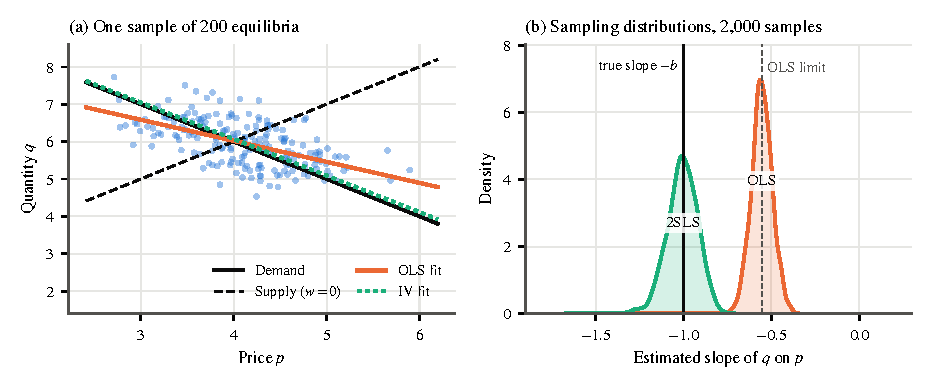
\includegraphics[width=\textwidth]{figures/appA/simultaneity.pdf}
\caption{Simultaneity bias and instrumental variables in a simulated market. Demand is
$q_t = 10 - p_t + u^d_t$ and supply is $q_t = 2 + p_t + w_t + u^s_t$, with $w_t \sim N(0, 1)$,
$u^d_t \sim N(0, 0.36)$ and $u^s_t \sim N(0, 0.25)$, all independent. (a) One sample of 200 equilibria with the
true demand curve and the supply curve at $w_t = 0$. The OLS fit has slope $-0.563$, and the IV fit with
instrument $w_t$ has slope $-0.977$. (b) Kernel densities of the OLS and two-stage least squares (2SLS, \cref{sec:A-2sls}) slopes over 2,000 samples of 200
markets. The solid line marks the demand slope $-1$ and the dashed line the OLS limit $-0.553$ from
\cref{prop:A-ols-simultaneity}. The mean first-stage $F$ statistic (\cref{sec:A-weakiv}) is 331. Seed 20261022, script
\texttt{sim\_iv.py}.}
\label{fig:A-simultaneity}
\end{figure}

\casehead{Order and rank conditions}
\Cref{cor:A-shifter} extends to any linear system. Let $y_t$ be a $G \times 1$ vector of endogenous variables
and $x_t$ an $M \times 1$ vector of exogenous variables with $\E[x_t x_t^\top]$ nonsingular. The structural
system is $B y_t + \Gamma x_t = u_t$, with $B$ nonsingular and $\E[x_t u_t^\top] = 0$. Its reduced form is
\begin{equation}\label{eq:A-system-rf}
y_t = \Pi x_t + v_t, \qquad \Pi = -B^{-1}\Gamma, \qquad v_t = B^{-1}u_t .
\end{equation}
The reduced-form coefficients are identified, $\Pi = \E[y_t x_t^\top]\E[x_t x_t^\top]^{-1}$, because $v_t$ is
uncorrelated with $x_t$. Consider one structural equation, normalized on its first endogenous variable:
\begin{equation}\label{eq:A-struct-eq}
y_{1t} = Y_{1t}^\top\beta + X_{1t}^\top\gamma + u_{1t} .
\end{equation}
It includes $G_1$ further endogenous variables $Y_{1t}$ and $M_1$ exogenous variables $X_{1t}$. The remaining
$M_2 = M - M_1$ exogenous variables $X_{2t}$ are excluded. Partition the reduced form conformably,
\begin{equation*}
y_{1t} = \pi_{11}^\top X_{1t} + \pi_{12}^\top X_{2t} + v_{1t}, \qquad
Y_{1t} = \Pi_{21}X_{1t} + \Pi_{22}X_{2t} + V_{1t},
\end{equation*}
where $\Pi_{22}$ is $G_1 \times M_2$. Substitute both into \eqref{eq:A-struct-eq}. The resulting identity holds
for all values of the exogenous variables, and the reduced-form errors are uncorrelated with them. Hence the
coefficients on $X_{1t}$ and $X_{2t}$ must match:
\begin{equation}\label{eq:A-rf-restrictions}
\pi_{11} = \Pi_{21}^\top\beta + \gamma, \qquad \pi_{12} = \Pi_{22}^\top\beta .
\end{equation}

\begin{proposition}[Rank and order conditions]\label{prop:A-rank}
The coefficients $(\beta, \gamma)$ of \eqref{eq:A-struct-eq} are identified if and only if
$\mathrm{rank}(\Pi_{22}) = G_1$. A necessary condition is $M_2 \ge G_1$, so the equation must exclude at least
as many exogenous variables as it includes endogenous variables on its right-hand side.
\end{proposition}

\begin{proof}
The second block of \eqref{eq:A-rf-restrictions} is a system of $M_2$ linear equations in the $G_1$ unknowns
$\beta$. If $\Pi_{22}^\top$ has full column rank $G_1$, the solution is unique:
\begin{equation*}
\beta = (\Pi_{22}\Pi_{22}^\top)^{-1}\Pi_{22}\,\pi_{12}, \qquad \gamma = \pi_{11} - \Pi_{21}^\top\beta .
\end{equation*}
If the rank is below $G_1$, pick $h \neq 0$ with $\Pi_{22}^\top h = 0$. The pair
$(\beta + h, \gamma - \Pi_{21}^\top h)$ also satisfies \eqref{eq:A-rf-restrictions}. The error it implies is
\begin{align*}
y_{1t} - Y_{1t}^\top(\beta + h) - X_{1t}^\top(\gamma - \Pi_{21}^\top h)
&= u_{1t} - h^\top\bigl(\Pi_{21}X_{1t} + \Pi_{22}X_{2t} + V_{1t}\bigr) + h^\top\Pi_{21}X_{1t} \\
&= u_{1t} - h^\top V_{1t} ,
\end{align*}
which is uncorrelated with $x_t$. The two coefficient vectors fit the same observables and satisfy the same
exogeneity restrictions, so the data cannot distinguish them. The order condition follows from
$\mathrm{rank}(\Pi_{22}) \le M_2$.
\end{proof}

In the market of \cref{cor:A-shifter}, demand includes one endogenous regressor (price) and excludes one
exogenous variable ($w_t$). The relevant reduced-form coefficient is $\Pi_{22} = -\frac{\delta}{b + c}$, which
is nonzero when $\delta \neq 0$, so demand is exactly identified. Supply excludes nothing, $M_2 = 0 < 1$, and
its slope remains unidentified until we observe a demand shifter.

\casehead{The link to conduct}
The same algebra explains why conduct is hard to identify (\cref{sec:03-identification}). In the linear model
of \cref{eq:03-linear-system}, the supply relation is $P_t = b_0 + \lambda Q_t + b_2 W_t + u^s_t$ with composite
slope $\lambda = b_1 - \frac{\theta}{a_1}$, where $\theta$ is conduct. An excluded demand shifter identifies
$\lambda$ by \cref{prop:A-rank}. The slope of marginal cost $b_1$ and conduct $\theta$ enter only through
$\lambda$. The Jacobian of the map from $(b_1, \theta)$ to the identified coefficients therefore has rank one,
and the two are not separately identified (\cref{prop:03-obs-equiv}). A demand rotator, a variable that changes
the slope of demand, makes the markup term move independently of quantity and restores identification
\citep{Bresnahan1982,Lau1982}. \Cref{sec:03-rotation} develops the argument.

\subsection{Potential outcomes and selection}\label{sec:A-potential}

Many questions in the book ask what an intervention does: a merger, a tax, entry by a rival. The
\emph{potential outcomes} framework states such questions precisely. Let $d_i \in \{0, 1\}$ indicate
treatment of unit $i$. The unit has two potential outcomes, $y_i(1)$ if treated and $y_i(0)$ if not, and we
observe only $y_i = d_i\,y_i(1) + (1 - d_i)\,y_i(0)$. The \emph{average treatment effect} is
$\mathrm{ATE} = \E[y_i(1) - y_i(0)]$, and the \emph{average treatment effect on the treated} is
$\mathrm{ATT} = \E[y_i(1) - y_i(0) \mid d_i = 1]$.

\begin{proposition}[Selection bias]\label{prop:A-selection}
The difference in mean outcomes between treated and untreated units satisfies
\begin{equation}\label{eq:A-selection}
\E[y_i \mid d_i = 1] - \E[y_i \mid d_i = 0]
= \mathrm{ATT} + \bigl\{\E[y_i(0) \mid d_i = 1] - \E[y_i(0) \mid d_i = 0]\bigr\} .
\end{equation}
\end{proposition}

\begin{proof}
Observed outcomes equal the relevant potential outcomes, so $\E[y_i \mid d_i = 1] = \E[y_i(1) \mid d_i = 1]$
and $\E[y_i \mid d_i = 0] = \E[y_i(0) \mid d_i = 0]$. Add and subtract $\E[y_i(0) \mid d_i = 1]$:
\begin{equation*}
\E[y_i(1) \mid d_i = 1] - \E[y_i(0) \mid d_i = 1] + \E[y_i(0) \mid d_i = 1] - \E[y_i(0) \mid d_i = 0] .
\end{equation*}
The first two terms form the ATT and the last two the bracket in \eqref{eq:A-selection}.
\end{proof}

The bracket is the \emph{selection bias}. It compares the untreated outcomes of two different groups, and it
is nonzero whenever the treated would have fared differently even without treatment. Random assignment makes
$d_i$ independent of $(y_i(1), y_i(0))$. The selection term then vanishes, and the ATT equals the ATE.

Selection is the central problem of merger retrospectives. Merging firms differ from non-merging ones, and
so do the rivals of merging firms. In hospital markets, non-merging hospitals whose rivals later merged had
price growth of $-2.9$ percent in 1985--1988, against $4.2$ percent for hospitals without merging rivals
\citep[p.~16]{Dafny2005}. A naive comparison would attribute part of this pre-existing gap to the mergers.
\Cref{sec:A-ivmodel} shows how an instrument removes it.

The same decomposition applies to continuous treatments. In the cross-industry regressions of the
structure-conduct-performance (SCP) paradigm, industry $k$ has a potential Lerner index $L_k(h)$ at each concentration level
$h$, and we observe $L_k = L_k(\HHI_k)$. Comparing industries at $h$ and $h'$,
\begin{multline*}
\E[L_k \mid \HHI_k = h] - \E[L_k \mid \HHI_k = h'] = \E[L_k(h) - L_k(h') \mid \HHI_k = h] \\
+ \bigl\{\E[L_k(h') \mid \HHI_k = h] - \E[L_k(h') \mid \HHI_k = h']\bigr\} .
\end{multline*}
The first term is a causal effect and the second a selection term, as in \cref{eq:01-potential-outcomes}.
Concentration is an equilibrium outcome of the same demand and cost primitives that determine margins, so
the selection term has no reason to vanish (\cref{sec:01-endogeneity}).

\casehead{Three empirical strategies on one industry}
The airline studies of \cref{ch:airlines} show three ways to overcome selection, each with its own
identifying assumption. \citet{Borenstein1989} runs reduced-form fare regressions on a carrier's route and
airport shares. His route-share effect is identified by an instrument, the carrier's share of endpoint
enplanements. He excludes it on the ground that fares respond to actual competition only
(\cref{sec:A-ivsources}). \citet{WhinstonCollins1992} run an event study of entry announcements. The value
effect of entry on incumbents is identified by the timing of news under efficient stock markets
(\cref{sec:A-eventstudy}). \citet{BerryCarnallSpiller2006} estimate a structural model of demand and
pricing.\footnote{We read NBER Working Paper 5561 (1996), \citet{BerryCarnallSpiller1996}, an earlier version of
their chapter. Page and table numbers marked WP refer to it.} Markups are identified by the estimated demand system together with an equilibrium assumption on
pricing. The three designs answer different questions, and their assumptions fail in different ways. A
related distinction is between prospective analysis, which predicts the effect of a change before it
happens, and retrospective analysis, which measures it afterwards (\cref{ch:mergers}). \Cref{sec:A-did}
develops the designs behind retrospectives.

\casehead{Partial identification}
When the assumptions needed for point identification are not credible, weaker assumptions often still bound
the feature of interest. \citet{HaileTamer2003} study English auctions in which bids need not equal values.
They assume only that bidders never bid more than their values and never let an opponent win at a price they
would have been willing to beat. These two inequalities bound the distribution of values from above and below.
\citet[pp.~493--499]{AradillasLopezGandhiQuint2013} allow symmetric private values with nonnegative dependence
when only the transaction price and the number of bidders are observed. The distribution of the highest value is then only partially
identified. If values are independent of the number of bidders, variation in that number across auctions tightens
the bounds on the seller's expected profit, the bidders' surplus and the optimal reserve price.
\Cref{ch:auction-empirics} develops both results, and \cref{sec:A-partialid} treats estimation and inference
for bounds.

\subsection{Monte Carlo experiments}\label{sec:A-montecarlo}

A \emph{Monte Carlo experiment} studies an estimator by applying it to data simulated from a known
data-generating process. It proceeds in four steps.
\begin{enumerate}[label=(\arabic*)]
\item Specify the data-generating process completely: functional forms, the true parameter $\theta_0$, the
  distributions of exogenous variables and errors, and the sample size $n$.
\item Fix the seed of the random number generator, so that the experiment can be reproduced exactly.
\item For $r = 1, \dots, R$, draw a sample and compute the estimate $\hat\theta_r$, its standard error and
  any test decision $D_r \in \{0, 1\}$, which equals one if the test rejects.
\item Summarize the $R$ replications.
\end{enumerate}
For a scalar parameter the usual summaries are the bias $\bar\theta - \theta_0$ with
$\bar\theta = \frac{1}{R}\sum_r\hat\theta_r$ and the standard deviation of $\hat\theta_r$ across replications.
Others are the \emph{root mean squared error}
$\mathrm{RMSE} = \bigl[\frac{1}{R}\sum_r(\hat\theta_r - \theta_0)^2\bigr]^{\frac{1}{2}}$, the coverage rate of
nominal confidence intervals, and the rejection rate $\frac{1}{R}\sum_r D_r$ of a test. Adding and
subtracting $\bar\theta$ inside the square gives
\begin{equation*}
\frac{1}{R}\sum_{r=1}^{R}(\hat\theta_r - \theta_0)^2
= (\bar\theta - \theta_0)^2 + \frac{1}{R}\sum_{r=1}^{R}(\hat\theta_r - \bar\theta)^2 ,
\end{equation*}
because the cross term $\frac{2}{R}(\bar\theta - \theta_0)\sum_r(\hat\theta_r - \bar\theta)$ is zero. The
squared RMSE is the squared bias plus the variance. Some estimators have no finite mean, such as
just-identified two-stage least squares (\cref{sec:A-weakiv}). For them the median and interquantile ranges
are more informative than the mean and the RMSE.

Monte Carlo summaries are estimates with their own sampling error. Consider a test whose true rejection
probability is $\alpha$. The replications are independent, so $\sum_r D_r$ is binomial with $R$ trials and
success probability $\alpha$. The estimated rejection rate $\hat\alpha = \frac{1}{R}\sum_r D_r$ therefore
satisfies
\begin{equation}\label{eq:A-mc-se}
\E[\hat\alpha] = \alpha, \qquad
\Var(\hat\alpha) = \frac{1}{R^2}\,R\,\alpha(1 - \alpha) = \frac{\alpha(1 - \alpha)}{R}, \qquad
\mathrm{se}(\hat\alpha) = \sqrt{\frac{\alpha(1 - \alpha)}{R}} .
\end{equation}
With $R = 10{,}000$ and $\alpha = 0.05$ the Monte Carlo standard error is 0.0022. A rejection rate of 0.058
then differs from 0.05 by more than three standard errors. In the same way, the Monte Carlo standard error
of $\bar\theta$ is the standard deviation across replications divided by $\sqrt{R}$.

The book uses such experiments to study SCP regressions on simulated Cournot industries
(\cref{sec:01-montecarlo}) and estimators of random-coefficient demand on simulated markets
(\cref{ch:blp,app:problems}). This appendix uses them throughout. They study instrumental variables
(\cref{fig:A-simultaneity,fig:A-weakiv}), latent regimes (\cref{fig:A-em}) and simulation estimators
(\cref{fig:A-simest}). They also study clustered inference (\cref{fig:A-cluster-mc}), kernel estimators
(\cref{fig:A-kde,fig:A-gpv}) and staggered difference in differences (\cref{fig:A-staggered}). Every one of
them reports its seed and the script that produced it.

\section{Least squares, panel data and systems}\label{sec:A-ols}

Ordinary least squares is the workhorse of empirical work, and it reappears inside almost every estimator
in the book. This section treats it as a projection, derives its large-sample behavior, lists the three
classic sources of bias, and develops the panel and system extensions used in the chapters.

\subsection{OLS as a projection}\label{sec:A-projection}

Let $(y_i, x_i)$ be independent and identically distributed, with $\E[y_i^2]$ finite and
$\E[x_i x_i^\top]$ finite and nonsingular. The \emph{linear projection} of $y_i$ on $x_i$ has coefficient
\begin{equation}\label{eq:A-projection}
\beta = \argmin_{b}\ \E\bigl[(y_i - x_i^\top b)^2\bigr] = \E[x_i x_i^\top]^{-1}\E[x_i y_i] .
\end{equation}
The second equality solves the first-order condition $\E[x_i(y_i - x_i^\top\beta)] = 0$. The
\emph{projection error} $e_i = y_i - x_i^\top\beta$ satisfies $\E[x_i e_i] = 0$ by construction. The
projection exists whether or not any economic model holds. A structural interpretation of $\beta$ is an
assumption: that the error of the economic model is uncorrelated with $x_i$, so the structural coefficient
coincides with the projection coefficient.

In a sample of size $n$, stack the observations into $y$ ($n \times 1$) and $X$ ($n \times K$) with full
column rank. The OLS estimator $\hat\beta = (X^\top X)^{-1}X^\top y$ solves the \emph{normal equations}
$X^\top(y - X\hat\beta) = 0$. Define the projection matrix $P_X = X(X^\top X)^{-1}X^\top$ and the
\emph{annihilator} $M_X = I_n - P_X$. Both are symmetric and idempotent, $M_X X = 0$, fitted values are
$P_X y$ and residuals are $\hat e = M_X y$.

\begin{theorem}[Frisch-Waugh-Lovell]\label{thm:A-fwl}
Partition $X = [X_1, X_2]$ and $\hat\beta = (\hat\beta_1^\top, \hat\beta_2^\top)^\top$ conformably, and let
$M_{X_2} = I_n - X_2(X_2^\top X_2)^{-1}X_2^\top$. Then
\begin{equation}\label{eq:A-fwl}
\hat\beta_1 = (X_1^\top M_{X_2} X_1)^{-1}X_1^\top M_{X_2} y = (\tilde X_1^\top\tilde X_1)^{-1}\tilde X_1^\top\tilde y,
\qquad \tilde X_1 = M_{X_2}X_1,\ \tilde y = M_{X_2} y ,
\end{equation}
and the residuals of the regression of $\tilde y$ on $\tilde X_1$ equal the residuals of the full regression.
\end{theorem}

\begin{proof}
The normal equations of the full regression are
\begin{equation*}
X_1^\top(y - X_1\hat\beta_1 - X_2\hat\beta_2) = 0, \qquad X_2^\top(y - X_1\hat\beta_1 - X_2\hat\beta_2) = 0 .
\end{equation*}
The second block gives $\hat\beta_2 = (X_2^\top X_2)^{-1}X_2^\top(y - X_1\hat\beta_1)$. Substituting,
\begin{equation*}
y - X_1\hat\beta_1 - X_2\hat\beta_2 = M_{X_2}(y - X_1\hat\beta_1) .
\end{equation*}
The first block becomes $X_1^\top M_{X_2}(y - X_1\hat\beta_1) = 0$, so
$\hat\beta_1 = (X_1^\top M_{X_2}X_1)^{-1}X_1^\top M_{X_2}y$. The inverse exists because $X$ has full column rank.
Since $M_{X_2}$ is symmetric and idempotent, $X_1^\top M_{X_2}X_1 = \tilde X_1^\top\tilde X_1$ and
$X_1^\top M_{X_2}y = \tilde X_1^\top\tilde y$. The full residual is $M_{X_2}(y - X_1\hat\beta_1) = \tilde y -
\tilde X_1\hat\beta_1$, which is the residual of the partialled regression.
\end{proof}

The theorem says that the coefficient on $X_1$ uses only the variation in $X_1$ that $X_2$ cannot explain.
The theorem underlies fixed effects (\cref{sec:A-panel}) and the control-function form of two-stage
least squares (\cref{sec:A-2sls}). It also justifies partialling out exogenous regressors
(\cref{sec:A-weakiv}) and concentrating out linear parameters (\cref{sec:A-gmm-computation}). The
double-residual estimator of the partially linear model (\cref{sec:A-plm}), the two-way fixed-effects
regression (\cref{sec:A-did-twfe}) and event-study dummies (\cref{sec:A-es-regression}) rest on it as well.

\subsection{Large-sample theory}\label{sec:A-ols-asy}

\begin{assumption}[Linear regression]\label{ass:A-ols}
\leavevmode
\begin{enumerate}[label=(\roman*)]
\item The observations $(y_i, x_i)$ are independent and identically distributed.
\item $y_i = x_i^\top\beta + e_i$ with $\E[x_i e_i] = 0$.
\item $Q = \E[x_i x_i^\top]$ is finite and nonsingular.
\item $\E\lVert x_i\rVert^4 < \infty$ and $\E[e_i^4] < \infty$.
\end{enumerate}
\end{assumption}

Part (iv) guarantees, by the Cauchy-Schwarz inequality, that $\Omega = \E[e_i^2x_ix_i^\top]$ is finite.

\begin{proposition}[Consistency and asymptotic normality of OLS]\label{prop:A-ols-asy}
Under \cref{ass:A-ols}, $\hat\beta \xrightarrow{p} \beta$ and
\begin{equation}\label{eq:A-ols-sandwich}
\sqrt{n}(\hat\beta - \beta) \xrightarrow{d} N\bigl(0,\ Q^{-1}\Omega Q^{-1}\bigr) .
\end{equation}
\end{proposition}

\begin{proof}
Substitute $y = X\beta + e$ into the estimator:
\begin{equation*}
\hat\beta - \beta = \Bigl(\frac{1}{n}X^\top X\Bigr)^{-1}\frac{1}{n}X^\top e
= \Bigl(\frac{1}{n}\sum_{i=1}^n x_ix_i^\top\Bigr)^{-1}\frac{1}{n}\sum_{i=1}^n x_ie_i .
\end{equation*}
By the weak law of large numbers, $\frac{1}{n}\sum_i x_ix_i^\top \xrightarrow{p} Q$ and
$\frac{1}{n}\sum_i x_ie_i \xrightarrow{p} \E[x_ie_i] = 0$. Matrix inversion is continuous at the nonsingular
$Q$, so the continuous mapping theorem gives $\hat\beta - \beta \xrightarrow{p} Q^{-1}\cdot 0 = 0$. For the
distribution, multiply by $\sqrt{n}$:
\begin{equation*}
\sqrt{n}(\hat\beta - \beta) = \Bigl(\frac{1}{n}\sum_{i=1}^n x_ix_i^\top\Bigr)^{-1}
\frac{1}{\sqrt{n}}\sum_{i=1}^n x_ie_i .
\end{equation*}
The terms $x_ie_i$ are independent with mean zero and finite variance $\Omega$, so the central limit theorem
gives $\frac{1}{\sqrt{n}}\sum_i x_ie_i \xrightarrow{d} N(0, \Omega)$. By Slutsky's theorem the product
converges to $Q^{-1}N(0, \Omega) = N(0, Q^{-1}\Omega Q^{-1})$.
\end{proof}

The variance in \eqref{eq:A-ols-sandwich} is called a \emph{sandwich} because $\Omega$ sits between two
copies of $Q^{-1}$. Under \emph{homoskedasticity}, $\E[e_i^2 \mid x_i] = \sigma^2$, the middle term becomes
$\Omega = \sigma^2Q$ and the variance collapses to $\sigma^2Q^{-1}$. Its conventional estimator is
$s^2(X^\top X)^{-1}$ with $s^2 = \frac{\hat e^\top\hat e}{n - K}$. Without homoskedasticity,
\citet{White1980} shows that
\begin{equation}\label{eq:A-hc0}
\hat V_{\mathrm{HC0}} = (X^\top X)^{-1}\Bigl(\sum_{i=1}^n\hat e_i^2x_ix_i^\top\Bigr)(X^\top X)^{-1}
\end{equation}
consistently estimates the variance of $\hat\beta$, in the sense that $n\hat V_{\mathrm{HC0}}
\xrightarrow{p} Q^{-1}\Omega Q^{-1}$. Finite-sample versions adjust the squared residuals, which are too
small on average. Let $h_{ii} = x_i^\top(X^\top X)^{-1}x_i$ be the \emph{leverage} of observation $i$. Under
homoskedasticity, $\hat e = M_Xe$ implies
\begin{equation*}
\E[\hat e_i^2 \mid X] = \sigma^2(M_X)_{ii} = \sigma^2(1 - h_{ii}) .
\end{equation*}
HC1 multiplies \eqref{eq:A-hc0} by $\frac{n}{n - K}$. HC2 replaces $\hat e_i^2$ by $\frac{\hat e_i^2}{1 - h_{ii}}$,
which is unbiased under homoskedasticity. HC3 uses $\frac{\hat e_i^2}{(1 - h_{ii})^2}$, which approximates the
jackknife and is conservative in small samples \citep{MacKinnonWhite1985}. In this book ``robust'' standard
errors mean heteroskedasticity-robust standard errors. They still assume independence across observations.
Clustered and serially correlated data need the estimators of \cref{sec:A-se}, which also covers heteroskedasticity
and autocorrelation consistent (HAC) estimators.

\subsection{Three sources of bias}\label{sec:A-bias}

OLS converges to the projection coefficient. It is biased for the structural coefficient whenever the
structural error is correlated with the regressors. Three mechanisms produce that correlation.

\casehead{Omitted variables}
Suppose $y_i = \beta_0 + \beta_1x_{1i} + \beta_2x_{2i} + e_i$ with $\E[e_i] = 0$ and $e_i$ uncorrelated with
both regressors, but we regress $y_i$ on a constant and $x_{1i}$ only. The short slope converges to
\begin{equation}\label{eq:A-ovb}
\frac{\Cov(y_i, x_{1i})}{\Var(x_{1i})}
= \frac{\beta_1\Var(x_{1i}) + \beta_2\Cov(x_{2i}, x_{1i}) + \Cov(e_i, x_{1i})}{\Var(x_{1i})}
= \beta_1 + \beta_2\,\frac{\Cov(x_{1i}, x_{2i})}{\Var(x_{1i})} .
\end{equation}
The bias is the effect of the omitted variable times the slope of its projection on the included one. With
vector regressors the bias is $\E[x_1x_1^\top]^{-1}\E[x_1x_2^\top]\beta_2$. In the firm-level regressions
that pit industry concentration against firm market share, omitting the share loads its effect onto
concentration whenever the two are correlated (\cref{sec:01-demsetz}).

\casehead{Measurement error}
Suppose $y_i = \beta_0 + \beta x_i^* + e_i$, but we observe $x_i = x_i^* + m_i$. The \emph{classical}
measurement error $m_i$ has mean zero and variance $\sigma_m^2$ and is uncorrelated with $x_i^*$ and $e_i$.
The OLS slope of $y_i$ on $x_i$ converges to
\begin{equation}\label{eq:A-attenuation}
\frac{\Cov(\beta_0 + \beta x_i^* + e_i,\ x_i^* + m_i)}{\Var(x_i^* + m_i)}
= \frac{\beta\Var(x_i^*)}{\Var(x_i^*) + \sigma_m^2} \equiv \beta\lambda .
\end{equation}
The \emph{reliability ratio} $\lambda \in (0, 1]$ is the share of the variance of the measured regressor that
is signal, so the slope is biased toward zero. Panel data with fixed effects can make this
\emph{attenuation} much worse \citep{GrilichesHausman1986}.

\begin{proposition}[Attenuation with fixed effects]\label{prop:A-fe-attenuation}
Let $y_{it} = \alpha_i + \beta x_{it}^* + e_{it}$ for $i = 1, \dots, n$ and $t = 1, \dots, T$, with $T$ fixed,
units independent, and $\E[e_{it} \mid x_{i1}^*, \dots, x_{iT}^*, \alpha_i] = 0$. We observe
$x_{it} = x_{it}^* + m_{it}$, where $m_{it}$ is independent across $i$ and $t$, has mean zero and variance
$\sigma_m^2$, and is independent of $\{x_{is}^*\}$, $\{e_{is}\}$ and $\alpha_i$. Define the within variance
$\Var_W(z) = \E\bigl[\frac{1}{T}\sum_t(z_{it} - \bar z_i)^2\bigr]$ with $\bar z_i = \frac{1}{T}\sum_t z_{it}$,
and suppose $\Var_W(x^*) > 0$. As $n \to \infty$ the within estimator converges to
\begin{equation}\label{eq:A-fe-attenuation}
\beta\lambda_W, \qquad
\lambda_W = \frac{\Var_W(x^*)}{\Var_W(x^*) + \frac{T - 1}{T}\sigma_m^2} .
\end{equation}
\end{proposition}

\begin{proof}
Write $\ddot z_{it} = z_{it} - \bar z_i$. The within transformation removes $\alpha_i$, so
$\ddot y_{it} = \beta\ddot x_{it}^* + \ddot e_{it}$, and the measured regressor is
$\ddot x_{it} = \ddot x_{it}^* + \ddot m_{it}$. The within estimator is
$\frac{\sum_i\sum_t\ddot x_{it}\ddot y_{it}}{\sum_i\sum_t\ddot x_{it}^2}$. Divide numerator and denominator by
$nT$ and apply the law of large numbers across units. The numerator converges to
$\beta\Var_W(x^*)$. The cross terms vanish because $m$ is independent of $x^*$ and $e$, and because strict
exogeneity makes $\E[\ddot x_{it}^*\ddot e_{it}] = 0$. The denominator converges to
$\Var_W(x^*) + \E\bigl[\frac{1}{T}\sum_t\ddot m_{it}^2\bigr]$. For each $t$,
\begin{equation*}
\E[\ddot m_{it}^2] = \Var(m_{it}) - 2\Cov(m_{it}, \bar m_i) + \Var(\bar m_i)
= \sigma_m^2 - \frac{2\sigma_m^2}{T} + \frac{\sigma_m^2}{T} = \frac{T - 1}{T}\,\sigma_m^2 .
\end{equation*}
The ratio of the two limits is \eqref{eq:A-fe-attenuation}.
\end{proof}

Compare $\lambda_W$ with the reliability ratio $\lambda = \frac{\Var(x^*)}{\Var(x^*) + \sigma_m^2}$ of a pooled
regression, which is valid if $\alpha_i$ is unrelated to the regressor. Inverting both ratios shows that
$\lambda_W < \lambda$ if and only if
\begin{equation*}
\frac{\Var_W(x^*)}{\Var(x^*)} < \frac{T - 1}{T} .
\end{equation*}
The left side is the share of the signal's variance that occurs within units. The right side is the same
share for independent noise. A persistent signal, whose variance is mostly between units, satisfies the
inequality easily. For example, if $x_{it}^* = a_i + \xi_{it}$ with independent $\xi_{it}$ of variance
$\sigma_\xi^2$ and $\Var(a_i) = \sigma_a^2$, then $\Var_W(x^*) = \frac{T - 1}{T}\sigma_\xi^2$ and
$\lambda_W = \frac{\sigma_\xi^2}{\sigma_\xi^2 + \sigma_m^2}$. This falls short of $\lambda$ whenever
$\sigma_a^2 > 0$. The result is the formal content of the critique that panel regressions of margins on
concentration with industry effects \citep{Salinger1990} can worsen attenuation
(\cref{prop:01-fe-attenuation}).

\casehead{Simultaneity}
\Cref{prop:A-ols-simultaneity} is the third mechanism. When the regressor is an equilibrium outcome, the
error of each equation moves it. Invalid instruments can bring the same bias back. With national demand
shocks, prices of the same brand in other cities are correlated with local demand errors. An instrumental
variables estimator built on them then ``is like doing ordinary least squares on a supply and demand
system'' \citep[p.~242]{Bresnahan1997}. \Cref{sec:A-ivmodel} gives the general formula, and
\cref{sec:10-bresnahan-iv} works out the cereal case.

\casehead{The structure-conduct-performance regression as a projection}
These mechanisms combine in the cross-industry regression of margins on concentration. Its OLS slope
converges to $\frac{\Cov(L_k, \HHI_k)}{\Var(\HHI_k)}$, a projection coefficient. Suppose every industry is a
symmetric Cournot industry, so $L_k = \frac{\HHI_k}{\varepsilon_k}$. If the elasticity $\varepsilon_k$ is
independent of $\HHI_k$, then $\Cov(L_k, \HHI_k) = \E[\frac{1}{\varepsilon_k}]\Var(\HHI_k)$, and the slope
converges to $\E[\frac{1}{\varepsilon_k}]$. Once elasticities, entry costs and conduct vary with
concentration, the slope mixes comparative statics with respect to several primitives and has no structural
meaning (\cref{prop:01-scp-plim}).

\subsection{Panel data}\label{sec:A-panel}

A \emph{panel} observes units $i = 1, \dots, n$ over periods $t = 1, \dots, T$. The basic model is
\begin{equation}\label{eq:A-panel}
y_{it} = x_{it}^\top\beta + \alpha_i + e_{it} ,
\end{equation}
where the unit effect $\alpha_i$ may be correlated with the regressors in any way. The key assumption is
\emph{strict exogeneity}, $\E[e_{it} \mid x_{i1}, \dots, x_{iT}, \alpha_i] = 0$: shocks in any period are
unrelated to the regressors in every period.

\casehead{Fixed effects}
Stack the data unit by unit and write $D = I_n \otimes \iota_T$ for the $nT \times n$ matrix of unit dummies,
where $\iota_T$ is a $T \times 1$ vector of ones. The \emph{fixed-effects}, or \emph{within}, estimator is OLS
of $y$ on $X$ and $D$. By \cref{thm:A-fwl} it equals OLS after premultiplying by
\begin{equation*}
M_D = I_{nT} - D(D^\top D)^{-1}D^\top = I_n \otimes \Bigl(I_T - \frac{1}{T}\iota_T\iota_T^\top\Bigr) ,
\end{equation*}
which subtracts each unit's time mean. Hence $\hat\beta_W = \bigl(\sum_i\sum_t\ddot x_{it}\ddot x_{it}^\top\bigr)^{-1}
\sum_i\sum_t\ddot x_{it}\ddot y_{it}$ with $\ddot z_{it} = z_{it} - \bar z_i$. It is consistent as $n \to \infty$
with $T$ fixed under strict exogeneity. Regressors that do not vary over time are swept out, and the error
variance is estimated with $nT - n - K$ degrees of freedom.

\casehead{First differences}
Differencing \eqref{eq:A-panel} also removes $\alpha_i$: $\Delta y_{it} = \Delta x_{it}^\top\beta + \Delta e_{it}$
for $t \ge 2$. OLS on the differences is consistent when $\E[\Delta x_{it}\Delta e_{it}] = 0$. With $T = 2$ the two
estimators coincide. The within deviations are $\ddot z_{i1} = -\frac{1}{2}\Delta z_{i2}$ and
$\ddot z_{i2} = \frac{1}{2}\Delta z_{i2}$, so
\begin{equation*}
\hat\beta_W = \Bigl(\sum_i 2\cdot\frac{1}{4}\Delta x_{i2}\Delta x_{i2}^\top\Bigr)^{-1}\sum_i 2\cdot\frac{1}{4}\Delta x_{i2}\Delta y_{i2}
= \Bigl(\sum_i\Delta x_{i2}\Delta x_{i2}^\top\Bigr)^{-1}\sum_i\Delta x_{i2}\Delta y_{i2} ,
\end{equation*}
which is the first-difference estimator. With $T > 2$ they differ, and their relative efficiency depends on
the serial correlation of $e_{it}$.

\casehead{Random effects}
If in addition $\E[\alpha_i \mid x_{i1}, \dots, x_{iT}] = 0$, the unit effect becomes part of a composite error
$\alpha_i + e_{it}$. With $\Var(\alpha_i) = \sigma_\alpha^2$ and homoskedastic, serially uncorrelated $e_{it}$,
the covariance matrix of unit $i$'s errors is $\Omega_i = \sigma_e^2I_T + \sigma_\alpha^2\iota_T\iota_T^\top$.
Write $\bar P = \frac{1}{T}\iota_T\iota_T^\top$ and $\bar Q = I_T - \bar P$. These are orthogonal idempotent
matrices, and
\begin{equation*}
\Omega_i = \sigma_e^2\bar Q + (\sigma_e^2 + T\sigma_\alpha^2)\bar P, \qquad
\sigma_e\,\Omega_i^{-\frac{1}{2}} = \bar Q + \phi\bar P = I_T - (1 - \phi)\bar P, \qquad
\phi = \frac{\sigma_e}{\sqrt{\sigma_e^2 + T\sigma_\alpha^2}} .
\end{equation*}
Generalized least squares is therefore OLS of $y_{it} - \vartheta\bar y_i$ on $x_{it} - \vartheta\bar x_i$ with
$\vartheta = 1 - \phi$. The \emph{random-effects} estimator replaces $\sigma_e^2$ and $\sigma_\alpha^2$ by estimates.
It quasi-demeans: $\vartheta = 0$ gives pooled OLS, and $\vartheta \to 1$ as
$\frac{T\sigma_\alpha^2}{\sigma_e^2} \to \infty$, so random effects approaches fixed effects in long panels
with large unit variance. It is efficient when its assumptions hold and inconsistent when $\alpha_i$ is
correlated with the regressors. \Cref{sec:A-spectests} tests between the two. \citet{FullerBattese1974}
extend the approach to crossed unit and time effects, $\alpha_i + \tau_t + e_{it}$.

\casehead{Two-way fixed effects}
Adding period effects gives $y_{it} = x_{it}^\top\beta + \alpha_i + \tau_t + e_{it}$. In a balanced panel,
\cref{thm:A-fwl} shows that the slope is OLS on the doubly demeaned data
$\ddot z_{it} = z_{it} - \bar z_{i\cdot} - \bar z_{\cdot t} + \bar z_{\cdot\cdot}$, the deviations from unit,
period and grand means. The variation that identifies $\beta$ differs across these estimators. Pooled OLS
uses all variation, including permanent differences across units. Fixed effects uses changes within units
over time. Two-way fixed effects uses changes within units relative to the average change in the same period,
so it is a difference-in-differences design with a continuous treatment (\cref{sec:A-did-twfe}).

\casehead{Application: tax pass-through in cigarettes}
\citet{Sumner1981} estimates the pass-through of state cigarette excise taxes into retail prices. His
equation (4) is $P_{it} = X_{it}\eta + \theta R_{it} + U_{it}$, with $i$ indexing states, $t$ years and
$R_{it}$ the tax per pack. Sumner's $\theta$ is the pass-through rate, which is neither conduct nor a generic
parameter. In the notation of \cref{eq:03-sumner-regression} it is
\begin{equation}\label{eq:A-sumner}
p_{sy} = \mu_s + \tau_y + \rho\,t_{sy} + e_{sy} ,
\end{equation}
with state effects $\mu_s$, year effects $\tau_y$ and pass-through rate $\rho$. The data are annual average
prices and taxes for 1954--1978 in 47 states and the District of Columbia. Alaska, Hawaii and New Hampshire
are excluded, which leaves 1,200 observations (pp.~1016--1017). Sumner's Table 1 reports three estimators of
$\rho$, each with its standard error. Two-way fixed effects by OLS gives 1.074 (0.013). Pooled OLS with the
national consumer price index in place of the year dummies and without state dummies gives 1.029 (0.011). A
variance-components estimator with random state and year effects \citep{FullerBattese1974} and the price index
gives 1.069 (0.013). The $R^2$ is about 0.99 with the dummies and 0.95 without them.

The comparison shows what each estimator uses. The pooled regression compares price levels across states
with permanently different taxes. Sumner notes that the three states with a large stake in tobacco growing
and cigarette manufacturing, North Carolina, Virginia and Kentucky, all have low taxes (fn.~8). State
dummies absorb such stable state characteristics (pp.~1015--1016), and the fixed-effects estimate rests on
changes in taxes within states over time. The random-effects estimate lies close to the fixed-effects one.
This is what quasi-demeaning predicts when $T = 25$ and the state variance component is large relative to
the idiosyncratic variance. The reported standard errors treat the 1,200 observations as independent.
\Cref{sec:A-sumner-se} recomputes them on a reconstructed panel, allowing for serial correlation within states
(\cref{tab:A-sumner}), and \cref{sec:A-did-twfe} reads the regression as a difference in differences with a
continuous treatment. \Cref{sec:03-sumner} discusses the economics of the test.

\subsection{Systems of equations}\label{sec:A-systems}

Many models in the book consist of several equations estimated together. Examples are the share
equations of a demand system, the residual demand curves of several firms, and the returns of several firms
around one event.

\casehead{Seemingly unrelated regressions}
Let $y_g = X_g\beta_g + e_g$ for equations $g = 1, \dots, G$, each with $n$ observations. Stack the equations
as $y = X\beta + e$, with $y = (y_1^\top, \dots, y_G^\top)^\top$ and $X = \diag(X_1, \dots, X_G)$ block diagonal.
Let $e_t = (e_{1t}, \dots, e_{Gt})^\top$ collect the errors of observation $t$, and assume $\E[e_te_t^\top] = \Sigma$
with independence across $t$. Then $\Var(e) = \Sigma \otimes I_n$. Generalized least squares gives the
\emph{seemingly unrelated regressions} (SUR) estimator of \citet{Zellner1962},
\begin{equation}\label{eq:A-sur}
\hat\beta_{SUR} = \bigl[X^\top(\Sigma^{-1}\otimes I_n)X\bigr]^{-1}X^\top(\Sigma^{-1}\otimes I_n)\,y .
\end{equation}
Feasible SUR replaces $\Sigma$ by $\hat\Sigma_{gh} = \frac{1}{n}\hat e_g^\top\hat e_h$ from equation-by-equation OLS
residuals. Iterating between $\hat\Sigma$ and $\hat\beta$ until convergence gives the Gaussian maximum likelihood
estimator.

\begin{proposition}[When SUR equals OLS]\label{prop:A-sur-ols}
If $X_g = X_0$ for every equation, or if $\Sigma$ is diagonal, then \eqref{eq:A-sur} equals equation-by-equation
OLS.
\end{proposition}

\begin{proof}
Use $(A \otimes B)(C \otimes D) = AC \otimes BD$ and $(A \otimes B)^{-1} = A^{-1} \otimes B^{-1}$. With
identical regressors, $X = I_G \otimes X_0$. Then
\begin{align*}
X^\top(\Sigma^{-1}\otimes I_n)X &= (I_G \otimes X_0^\top)(\Sigma^{-1}\otimes I_n)(I_G \otimes X_0)
= \Sigma^{-1}\otimes X_0^\top X_0 ,\\
X^\top(\Sigma^{-1}\otimes I_n)\,y &= (\Sigma^{-1}\otimes X_0^\top)\,y .
\end{align*}
The inverse of the first matrix is $\Sigma \otimes (X_0^\top X_0)^{-1}$, so
\begin{equation*}
\hat\beta_{SUR} = \bigl[\Sigma \otimes (X_0^\top X_0)^{-1}\bigr](\Sigma^{-1}\otimes X_0^\top)\,y
= \bigl[I_G \otimes (X_0^\top X_0)^{-1}X_0^\top\bigr]y ,
\end{equation*}
which stacks the OLS regressions of each $y_g$ on $X_0$. If $\Sigma = \diag(\sigma_1^2, \dots, \sigma_G^2)$,
both $X^\top(\Sigma^{-1}\otimes I_n)X$ and $X^\top(\Sigma^{-1}\otimes I_n)y$ are block diagonal with blocks
$\sigma_g^{-2}X_g^\top X_g$ and $\sigma_g^{-2}X_g^\top y_g$. The weights cancel equation by equation, leaving
$(X_g^\top X_g)^{-1}X_g^\top y_g$.
\end{proof}

SUR gains precision only when the errors are correlated across equations and the regressors differ. It
becomes indispensable when coefficients are restricted across equations. The linear approximate almost ideal demand
system is a leading case of identical regressors. Every share equation contains the same log prices and the same log
total expenditure deflated by the Stone index. Without cross-equation restrictions, OLS equation by equation therefore
coincides with SUR (\cref{sec:05-stone}).

\casehead{Adding up and cross-equation restrictions}
Budget shares sum to one, so the errors of a complete share system sum to zero for every observation, and
$\Sigma$ is singular. We drop one equation and recover its coefficients from the adding-up restrictions. The
maximum likelihood (iterated SUR) estimates do not depend on which equation is dropped \citep{Barten1969}.
Symmetry and homogeneity restrictions take the linear form $R\beta = r$. Restricted GLS minimizes
$(y - Xb)^\top W(y - Xb)$ subject to $Rb = r$, with $W = \Sigma^{-1}\otimes I_n$. The Lagrangian first-order
condition $-2X^\top W(y - Xb) + 2R^\top\ell = 0$ gives $b = \hat\beta - VR^\top\ell$ with
$V = (X^\top WX)^{-1}$. Imposing $Rb = r$ determines the multiplier $\ell$:
\begin{equation}\label{eq:A-restricted-gls}
\tilde\beta = \hat\beta - VR^\top\bigl(RVR^\top\bigr)^{-1}\bigl(R\hat\beta - r\bigr) .
\end{equation}

\casehead{Which restrictions can be tested}
\citet[Section~3.3, pp.~67--70]{DeatonMuellbauer1980b} use the Rotterdam model to sort the restrictions of demand
theory by how they can be tested. For goods $g = 1, \dots, G$ and periods $t$, the model is
\begin{equation}\label{eq:A-rotterdam}
\bar w_{gt}\,\Delta\ln q_{gt} = b_g\,\Delta\ln\bar x_t + \sum_{h=1}^{G}c_{gh}\,\Delta\ln p_{ht} + e_{gt},
\qquad \Delta\ln\bar x_t = \sum_{h=1}^{G}\bar w_{ht}\,\Delta\ln q_{ht}
\end{equation}
(their eqs.~3.3 and~3.4). Here $\bar w_{gt}$ is the budget share used in the discrete approximation to the
differentials. It is chosen so that the identity for $\Delta\ln\bar x_t$ holds in the data (p.~69). The variable
$\Delta\ln\bar x_t$ is the change in real total expenditure, and $b_g$ is the marginal budget share. The coefficient
$c_{gh} = \frac{p_gp_hs_{gh}}{x}$ is a compensated price effect, where $s_{gh}$ is the Slutsky term and $x$ is total
expenditure (their eqs.~3.5 and~3.6). The coefficients are treated as constants. Adding up requires
$\sum_gb_g = 1$ and $\sum_gc_{gh} = 0$ for every $h$ (their eq.~3.7). Homogeneity requires $\sum_hc_{gh} = 0$ for
every $g$, and symmetry requires $c_{gh} = c_{hg}$ (eqs.~3.8 and~3.9). The three restrictions differ in how they
can be tested.

\begin{proposition}[Adding up holds by construction]\label{prop:A-addingup}
Let $y_g = X_0\beta_g + e_g$ for $g = 1, \dots, G$, with common regressors $X_0$ of full column rank. Suppose the
data satisfy $\sum_gy_g = X_0a$ for a known vector $a$. Then the OLS estimates satisfy $\sum_g\hat\beta_g = a$, and
for every observation the OLS residuals sum to zero across equations.
\end{proposition}

\begin{proof}
OLS is linear in the dependent variable, so
\begin{equation*}
\sum_{g=1}^{G}\hat\beta_g = (X_0^\top X_0)^{-1}X_0^\top\sum_{g=1}^{G}y_g = (X_0^\top X_0)^{-1}X_0^\top X_0\,a = a .
\end{equation*}
The residuals then sum to $\sum_gy_g - X_0\sum_g\hat\beta_g = X_0a - X_0a = 0$.
\end{proof}

In \eqref{eq:A-rotterdam} every equation has the same regressors, and the left-hand sides sum to
$\Delta\ln\bar x_t$, the first regressor. The proposition applies with $a$ the first unit vector. OLS therefore
gives $\sum_g\hat b_g = 1$ and $\sum_g\hat c_{gh} = 0$ whatever the data. Adding up cannot be tested, and it places
no restriction on the explanatory power of the equations (p.~69). Homogeneity involves the coefficients of one
equation only. It can be imposed and tested equation by equation, with a $t$ or $F$ test of $\sum_hc_{gh} = 0$.
Symmetry links pairs of equations, so it needs the system, estimated by \eqref{eq:A-restricted-gls} with one
equation dropped. The restrictions are also nested. Under adding up, symmetry gives
$\sum_hc_{gh} = \sum_hc_{hg} = 0$ for every $g$, so symmetry implies homogeneity. Tests of symmetry therefore come
after tests of homogeneity, and \cref{sec:A-wald} reports their outcome. Negativity, the requirement that the matrix
$C = (c_{gh})$ be negative semidefinite, is an inequality restriction and needs other tools.

\Cref{sec:05-estimation} applies these tools to the almost ideal demand system. \citet{Hausman1997}
combines SUR with instruments to estimate brand demand for cereal, a form of three-stage least squares
(\cref{sec:A-3sls,sec:10-hausman-identification}). In event studies with several firms and a common event
date, SUR accounts for the contemporaneous correlation of returns in tests across firms \citep[pp.~172--173]{Binder1985}.
\Citet{WhinstonCollins1992} use it in this way (\cref{sec:A-eventstudy,sec:09-wc}).

\subsection{Testing linear restrictions}\label{sec:A-wald}

Consider $q$ linear restrictions $H_0\colon R\beta = r$, with $R$ a $q \times K$ matrix of rank $q$. Let
$\hat V$ estimate the variance of $\hat\beta$, for example $\frac{1}{n}$ times a consistent estimator of the
asymptotic variance in \eqref{eq:A-ols-sandwich}. The \emph{Wald statistic} is
\begin{equation}\label{eq:A-wald}
\mathcal{W} = (R\hat\beta - r)^\top\bigl[R\hat VR^\top\bigr]^{-1}(R\hat\beta - r) \xrightarrow{d} \chi^2_q
\quad\text{under } H_0 .
\end{equation}
The limit follows in two steps. Under $H_0$, $\sqrt{n}(R\hat\beta - r) = R\sqrt{n}(\hat\beta - \beta)
\xrightarrow{d} N(0, RVR^\top)$ by \cref{prop:A-ols-asy}. If $\zeta \sim N(0, \Sigma_\zeta)$ is $q$-dimensional
with $\Sigma_\zeta$ nonsingular, then $\Sigma_\zeta^{-\frac{1}{2}}\zeta \sim N(0, I_q)$, so
$\zeta^\top\Sigma_\zeta^{-1}\zeta$ is a sum of $q$ squared independent standard normals. Slutsky's theorem
handles the estimated variance. With homoskedastic normal errors and the conventional variance estimator,
$\frac{\mathcal{W}}{q}$ equals
\begin{equation*}
F = \frac{\frac{1}{q}(\mathrm{SSR}_r - \mathrm{SSR}_u)}{\frac{1}{n - K}\mathrm{SSR}_u} \sim F(q, n - K) ,
\end{equation*}
where $\mathrm{SSR}_r$ and $\mathrm{SSR}_u$ are the restricted and unrestricted sums of squared residuals. The
\emph{Chow test} of equal coefficients in two groups is the special case in which the unrestricted model
estimates each group separately \citep{Chow1960a}.

Four applications illustrate the range of uses.
\begin{itemize}
\item \citet{GenesoveMullin1998} test whether the price coefficient and intercept of sugar demand are equal
  across seasons.\footnote{We read the working-paper version of \citet{GenesoveMullin1998}. Equation, table and
  page numbers marked WP refer to it. Printed page numbers are those on the pages of that version.} With
  Newey-West standard errors, the $\chi^2_{(2)}$ statistics are 6.90, 28.18, 29.17 and 25.96 for quadratic,
  linear, log-linear and exponential demand (WP Table~6, p.~29). All exceed the 5 percent cutoff of 5.99, so
  demand rotates between seasons (\cref{tab:03-gm-demand}). A pooled specification with a time trend tests
  instead that the high-season shifts in intercept and slope are both zero. Its statistics are 4.91, 22.73,
  23.40 and 20.77 (WP Table~5, p.~28). The quadratic form does not reject there, so for that form the
  conclusion depends on the specification.
\item The revenue test of \citet{PanzarRosse1987} restricts a single linear combination, the sum
  $\hat\psi = \sum_k\hat\beta_k$ of factor-price elasticities of revenue. With $R = \iota^\top$, the statistic
  is $t = \frac{\hat\psi - \psi_0}{\sqrt{\iota^\top\hat V\iota}}$. Long-run competition implies $\psi = 1$, a
  two-sided test. Monopoly implies $\psi \le 0$, and we reject it at 5 percent when $\frac{\hat\psi}{\mathrm{se}}
  > 1.645$ (\cref{sec:03-panzar-rosse}).
\item \citet[pp.~353--354]{Borenstein1989} rejects a common constant across airlines but fails to reject
  common slopes, so his fare equations pool the slopes and keep carrier effects. A Chow test does not reject
  equal route-share effects across the 20th, 50th and 80th fare percentiles, while it rejects a common
  coefficient on flight frequency (p.~358 and fn.~41). The three percentile regressions use the same routes,
  so a test across them must account for the covariance of their estimates, as a stacked or SUR regression
  does.
\item Tests of demand theory apply the same logic to systems. \citet{Barten1969} estimated the Rotterdam model
  \eqref{eq:A-rotterdam} for 16 groups of Dutch consumption by maximum likelihood, with intercepts for gradual
  changes in tastes. Imposing homogeneity caused ``a very large drop in the value of the maximized likelihood,
  much larger than could conceivably have arisen by chance'' \citep[pp.~69--70]{DeatonMuellbauer1980b}. Symmetry
  was rejected as well, but \citet{Deaton1972} gives technical grounds for doubting that test. \citet{Deaton1974}
  found the same pattern for nine groups of British data from 1900 to 1970. Homogeneity was rejected, while
  symmetry as an additional restriction was not particularly damaging \citep[p.~70]{DeatonMuellbauer1980b}. The
  likelihood ratio statistic used in these studies is asymptotically equivalent to $\mathcal{W}$ under $H_0$
  (\cref{thm:A-trinity}). Each
  rejection is joint, of the theory and of a functional form. Deaton and Muellbauer stress that the Rotterdam,
  double-log and translog systems all reject, at least on aggregate data (pp.~72--74).
\end{itemize}

\section{Instrumental variables}\label{sec:A-iv}

Instrumental variables (IV) are the book's main tool for endogenous regressors: prices in demand equations,
quantities in supply relations, market shares in fare equations and mergers in price regressions. This
section develops the linear model and two-stage least squares, then the special problems of nonlinear models
and weak instruments. It closes with specification tests, heterogeneous effects and system estimation.

\subsection{The IV model}\label{sec:A-ivmodel}

\begin{assumption}[Linear instrumental variables]\label{ass:A-iv}
The observations $(y_i, x_i, z_i)$ are independent and identically distributed, with $x_i$ of dimension $K$
and $z_i$ of dimension $L \ge K$, and
\begin{equation}\label{eq:A-iv-model}
y_i = x_i^\top\beta + e_i .
\end{equation}
\begin{enumerate}[label=(\roman*)]
\item The instruments are exogenous, $\E[z_ie_i] = 0$.
\item The instruments are relevant, $\mathrm{rank}\,\E[z_ix_i^\top] = K$.
\item $\E[z_iz_i^\top]$ is finite and nonsingular, and $\E\lVert z_i\rVert^4$, $\E\lVert x_i\rVert^4$ and $\E[e_i^4]$
  are finite.
\end{enumerate}
\end{assumption}

Exogenous regressors, such as the constant, appear in both $x_i$ and $z_i$. They serve as their own
instruments and are called \emph{included instruments}. The other elements of $z_i$ are the \emph{excluded
instruments}. Exogeneity of an excluded instrument combines two claims. The instrument is unrelated to the
unobserved determinants of the outcome, and it affects the outcome only through $x_i$, which is the
\emph{exclusion restriction}. Relevance requires the excluded instruments to predict every endogenous
regressor beyond what the included instruments predict. In the just-identified case $L = K$, exogeneity gives
$\beta = \E[z_ix_i^\top]^{-1}\E[z_iy_i]$, and the IV estimator is its sample analogue
$\hat\beta_{IV} = (Z^\top X)^{-1}Z^\top y$.

\casehead{Indirect least squares}
Let $y_i = \beta_0 + \beta_1x_i + e_i$ with one instrument $z_i$ and a constant. Exogeneity gives
$\Cov(z_i, y_i) = \beta_1\Cov(z_i, x_i) + \Cov(z_i, e_i) = \beta_1\Cov(z_i, x_i)$, so
\begin{equation}\label{eq:A-ils}
\beta_1 = \frac{\Cov(z_i, y_i)}{\Cov(z_i, x_i)}
= \frac{\frac{\Cov(z_i, y_i)}{\Var(z_i)}}{\frac{\Cov(z_i, x_i)}{\Var(z_i)}} = \frac{\rho_1}{\pi_1} .
\end{equation}
Here $\pi_1$ is the slope of the \emph{first stage}, the regression of $x_i$ on $z_i$. The slope of the
\emph{reduced form}, the regression of $y_i$ on $z_i$, is $\rho_1$. The IV estimand is the reduced-form effect of the
instrument divided by its first-stage effect. The identity also holds exactly in the sample, because each
estimator is a ratio of sample covariances. Estimating $\beta_1$ this way is called \emph{indirect least
squares}. With exogenous controls, \cref{thm:A-fwl} shows that the identity holds after the controls are
partialled out of $y_i$, $x_i$ and $z_i$.

\casehead{The Wald estimator}
If $z_i$ is binary with $p = \Pr(z_i = 1)$, then
\begin{align*}
\Cov(z_i, y_i) &= \E[z_iy_i] - \E[z_i]\E[y_i] \\
&= p\,\E[y_i \mid z_i = 1] - p\bigl(p\,\E[y_i \mid z_i = 1] + (1 - p)\,\E[y_i \mid z_i = 0]\bigr) \\
&= p(1 - p)\bigl(\E[y_i \mid z_i = 1] - \E[y_i \mid z_i = 0]\bigr) .
\end{align*}
The same algebra applies to $x_i$, and \eqref{eq:A-ils} becomes the \emph{Wald estimator}
\begin{equation}\label{eq:A-wald-estimator}
\beta_1 = \frac{\E[y_i \mid z_i = 1] - \E[y_i \mid z_i = 0]}{\E[x_i \mid z_i = 1] - \E[x_i \mid z_i = 0]} .
\end{equation}

\casehead{Invalid instruments}
If the instrument is correlated with the error, the same algebra gives
\begin{equation}\label{eq:A-iv-bias}
\plim\hat\beta_{1,IV} - \beta_1 = \frac{\Cov(z_i, e_i)}{\Cov(z_i, x_i)}
= \frac{\Corr(z_i, e_i)}{\Corr(z_i, x_i)}\cdot\frac{\sigma_e}{\sigma_x} .
\end{equation}
The OLS bias is $\frac{\Cov(x_i, e_i)}{\Var(x_i)} = \Corr(x_i, e_i)\frac{\sigma_e}{\sigma_x}$, so the ratio of the
two biases is
\begin{equation*}
\frac{\plim\hat\beta_{1,IV} - \beta_1}{\plim\hat\beta_{1,OLS} - \beta_1}
= \frac{\Corr(z_i, e_i)}{\Corr(x_i, e_i)\,\Corr(z_i, x_i)} .
\end{equation*}
A weak instrument puts a small $\Corr(z_i, x_i)$ in the denominator. It magnifies even a slight correlation
with the error, and IV can then be more biased than OLS. Weak and slightly invalid instruments are a
dangerous mix. Bresnahan's critique of prices in other cities as instruments is an example. National demand
shocks make $\Cov(z_i, e_i)$ positive, and the larger their share of price variation, the closer the IV bias
comes to the OLS bias (\cref{sec:10-bresnahan-iv}). With a valid and strong instrument, by contrast, 2SLS is
centered on the truth, as panel (b) of \cref{fig:A-simultaneity} shows.

\casehead{Application: rival mergers and hospital prices}
\citet{Dafny2009} estimates the effect of hospital mergers on prices.\footnote{Numbers and page references
follow the NBER working-paper version, revised in October 2007 \citep{Dafny2005}. Table numbers refer to that
version.} A comparison of merging with non-merging hospitals suffers from selection, because hospitals that
merge differ in unobserved ways from those that do not. Following \citet{Eckbo1983}, she studies the
\emph{rivals} of merging hospitals instead. If prices are strategic complements, rivals raise their prices
after a merger as well. Exposure to a rival's merger is still selected, because markets with mergers differ
from markets without them, so she instruments for it.

The data combine 97 independent mergers between 1989 and 1996, in which two hospitals consolidated into a
single licensed entity \citep{DranoveLindrooth2003}, with Medicare cost reports for 1985--2000 (pp.~12--15).
The price of a hospital is its inpatient revenue per case-mix-adjusted non-Medicare discharge. The estimation
sample contains 877 non-merging hospitals with at least two rivals within 7 miles. The treatment $R_i$ is the
number of rival mergers within 7 miles between 1989 and 1996, with mean 0.156 (Table 1). The outcome is price
growth over the merger wave, $\Delta\ln p_i = \ln p_{i,1997} - \ln p_{i,1988}$, with mean 0.010. The instrument
$C_i$ is the number of \emph{co-located} rival pairs, meaning pairs of rivals within 0.3 miles and at most five
blocks of each other in 1988. The estimating equations are
\begin{align}
R_i &= \pi_0 + \pi_1C_i + w_i^\top\pi_2 + v_i && \text{(first stage)}, \label{eq:A-dafny-fs}\\
\Delta\ln p_i &= \rho_0 + \rho_1C_i + w_i^\top\rho_2 + \varepsilon_i && \text{(reduced form)}, \label{eq:A-dafny-rf}\\
\Delta\ln p_i &= \beta_0 + \beta_1R_i + w_i^\top\beta_2 + e_i && \text{(structural equation)}. \label{eq:A-dafny-iv}
\end{align}
The controls $w_i$ include hospital characteristics: ownership, teaching status, Medicaid share,
debt-to-asset ratio, occupancy and bed-size categories. They also include market characteristics, namely
population categories, the penetration of health maintenance organizations and log income per capita, with or
without state fixed effects.

Relevance has an economic rationale. Co-located hospitals can save more by closing duplicate departments,
and they gain more market power from merging, because location is a primary source of differentiation in
inpatient care (p.~3). In the data, co-located hospitals merge at a rate of 11.0 percent, against 3.7 percent
for other hospitals (p.~18). Exclusion requires that rival co-location affect price growth only through rival
mergers. Dafny names the main threat. Before 1988, new hospitals might have entered next to existing ones in
areas where prices were expected to rise. She argues that this is unlikely, because there has been very
little entry into acute care since the Hill-Burton Act of 1946 (fn.~27).

\Cref{tab:A-dafny} reproduces the main results. One more co-located rival pair raises the number of rival
mergers by 0.119, large relative to the mean of 0.156, with a $t$-statistic of about 6.6. It raises price
growth by 0.045, against a mean of 0.010. Because the model is exactly identified, the IV estimate is the ratio
\eqref{eq:A-ils}. The rounded coefficients give $\frac{0.045}{0.119} = 0.378$, and the unrounded ones give the
reported 0.376 (fn.~29). The implied price increase is $e^{0.376} - 1 = 46$ percent, or 35 percent with state
fixed effects (fn.~30). OLS finds no effect, with an estimate of 0.016 and a standard error of 0.026. The sign
of the OLS bias matches the pre-period evidence of \cref{sec:A-potential}. Hospitals later exposed to rival
mergers had lower price growth before the merger wave, so treating rival mergers as exogenous understates
their effect.

\begin{table}[htbp]
\centering
\caption{Rival mergers and hospital price growth: first stage, reduced form, IV and OLS}
\label{tab:A-dafny}
\small
\begin{tabular}{@{}lcc@{}}
\toprule
 & Without state effects & With state effects \\
\midrule
\multicolumn{3}{@{}l}{\textit{A. First stage (OLS)}} \\
Own merger on own co-location ($N = 4{,}487$) & 0.066 & 0.062 \\
 & (0.016) & (0.016) \\
Rival mergers on co-located rival pairs ($N = 877$) & 0.119 & 0.112 \\
 & (0.018) & (0.019) \\
\addlinespace
\multicolumn{3}{@{}l}{\textit{B. Reduced form: log price growth on co-located rival pairs (OLS)}} \\
1985--1988, before the merger wave ($N = 877$) & $-0.016$ & $-0.013$ \\
 & (0.010) & (0.011) \\
1988--1997, merger period ($N = 877$) & 0.045 & 0.034 \\
 & (0.014) & (0.015) \\
1997--2000, after the merger wave ($N = 703$) & $-0.008$ & $-0.001$ \\
 & (0.013) & (0.014) \\
\addlinespace
\multicolumn{3}{@{}l}{\textit{C. Log price growth 1988--1997 on the number of rival mergers ($N = 877$)}} \\
IV, instrument: co-located rival pairs & 0.376 & 0.301 \\
 & (0.132) & (0.147) \\
OLS & 0.016 & $-0.003$ \\
 & (0.026) & (0.027) \\
\bottomrule
\end{tabular}

\smallskip
\begin{minipage}{0.92\textwidth}\footnotesize
Notes: Standard errors in parentheses. Every regression controls for the hospital and market characteristics
listed in the text. The own-merger regression is a linear probability model on all 4,487 hospitals. The other
rows use non-merging hospitals with at least two rivals within 7 miles. Price is inpatient revenue per
case-mix-adjusted non-Medicare discharge, and price changes are censored at the 5th and 95th percentiles.
Source: \citet{Dafny2005}, Table 2 (panel A), Table 3 (panel B) and Table 4 (panel C).
\end{minipage}
\end{table}

Several checks support the design. Rival co-location predicts price growth neither before nor after the
merger wave (panel B), so co-located markets were not on steeper price paths. The IV estimate barely moves
when all controls are dropped, at 0.352 (0.132) (Appendix Table 1). It more than doubles when the market
radius shrinks to 5 miles, at 0.962 (0.377), and it vanishes at 10 miles, at 0.051 (0.054) (Table 5). Effects
that fade with distance are what a local market-power mechanism predicts. Two further checks appear below. An
overidentification test with two distance bands does not reject (\cref{sec:A-spectests}). Using fitted values
from a nonlinear first stage as the instrument gives a smaller but significant estimate
(\cref{sec:A-nonlinear-iv}). The estimate is local to the mergers that the instrument moves, which are mergers
of co-located hospitals with especially large gains in market power (p.~26 and \cref{sec:A-late}).
\Cref{sec:11-dafny} develops the economics.

\subsection{Two-stage least squares}\label{sec:A-2sls}

With more instruments than regressors, $L > K$, the sample moment conditions $\frac{1}{n}Z^\top(y - Xb) = 0$ have
no exact solution. \emph{Two-stage least squares} (2SLS) uses the linear combinations of the instruments that
best predict the regressors. Let $P_Z = Z(Z^\top Z)^{-1}Z^\top$ and $\hat X = P_ZX$. The estimator is
\begin{equation}\label{eq:A-2sls}
\hat\beta_{2SLS} = (X^\top P_ZX)^{-1}X^\top P_Zy .
\end{equation}
Three routes lead to \eqref{eq:A-2sls}.
\begin{enumerate}[label=(\alph*)]
\item The first route regresses each column of $X$ on $Z$ and then regresses $y$ on the fitted values $\hat X$.
  Because $P_Z$ is symmetric and idempotent, $(\hat X^\top\hat X)^{-1}\hat X^\top y = (X^\top P_ZX)^{-1}X^\top P_Zy$.
  Exogenous regressors are among the instruments, so their fitted values equal themselves.
\item The second route uses $\hat X$ as instruments in the just-identified IV formula:
  $(\hat X^\top X)^{-1}\hat X^\top y = (X^\top P_ZX)^{-1}X^\top P_Zy$.
\item The third route minimizes the quadratic form $(y - Xb)^\top Z(Z^\top Z)^{-1}Z^\top(y - Xb)$ in the moment
  conditions. Its first-order condition $-2X^\top Z(Z^\top Z)^{-1}Z^\top(y - Xb) = 0$ gives \eqref{eq:A-2sls}. This is
  the generalized method of moments with weighting matrix $(Z^\top Z)^{-1}$ (\cref{eq:A-linear-gmm} in \cref{sec:A-gmm-asy}).
\end{enumerate}
When $L = K$, $Z^\top X$ is square and invertible, and
\begin{align*}
(X^\top Z(Z^\top Z)^{-1}Z^\top X)^{-1}X^\top Z(Z^\top Z)^{-1}Z^\top y
&= (Z^\top X)^{-1}(Z^\top Z)(X^\top Z)^{-1}X^\top Z(Z^\top Z)^{-1}Z^\top y \\
&= (Z^\top X)^{-1}Z^\top y ,
\end{align*}
so 2SLS reduces to IV. In particular, a just-identified estimate does not depend on which linear
combination of the instruments is used.

\begin{proposition}[Asymptotics of 2SLS]\label{prop:A-2sls-asy}
Under \cref{ass:A-iv}, let $Q_{zx} = \E[z_ix_i^\top]$, $Q_{zz} = \E[z_iz_i^\top]$, $\Omega = \E[e_i^2z_iz_i^\top]$ and
$H = Q_{zx}^\top Q_{zz}^{-1}Q_{zx}$. Then $\hat\beta_{2SLS} \xrightarrow{p} \beta$ and
\begin{equation}\label{eq:A-2sls-avar}
\sqrt{n}(\hat\beta_{2SLS} - \beta) \xrightarrow{d}
N\bigl(0,\ H^{-1}Q_{zx}^\top Q_{zz}^{-1}\,\Omega\,Q_{zz}^{-1}Q_{zx}H^{-1}\bigr) .
\end{equation}
Under conditional homoskedasticity, $\E[e_i^2 \mid z_i] = \sigma^2$, the variance reduces to $\sigma^2H^{-1}$.
\end{proposition}

\begin{proof}
Substituting $y = X\beta + e$ into \eqref{eq:A-2sls},
\begin{equation*}
\hat\beta_{2SLS} - \beta = \Bigl[\frac{X^\top Z}{n}\Bigl(\frac{Z^\top Z}{n}\Bigr)^{-1}\frac{Z^\top X}{n}\Bigr]^{-1}
\frac{X^\top Z}{n}\Bigl(\frac{Z^\top Z}{n}\Bigr)^{-1}\frac{Z^\top e}{n} .
\end{equation*}
By the law of large numbers, $\frac{Z^\top X}{n} \xrightarrow{p} Q_{zx}$, $\frac{Z^\top Z}{n} \xrightarrow{p} Q_{zz}$ and
$\frac{Z^\top e}{n} \xrightarrow{p} \E[z_ie_i] = 0$. Relevance makes $H$ nonsingular, because $Q_{zx}$ has rank $K$
and $Q_{zz}^{-1}$ is positive definite. The continuous mapping theorem gives consistency. Multiplying by
$\sqrt{n}$ replaces $\frac{Z^\top e}{n}$ by $\frac{1}{\sqrt{n}}\sum_iz_ie_i$, which converges in distribution to
$N(0, \Omega)$ by the central limit theorem. Slutsky's theorem gives \eqref{eq:A-2sls-avar}. Under
homoskedasticity $\Omega = \sigma^2Q_{zz}$, and the sandwich collapses to $\sigma^2H^{-1}HH^{-1} = \sigma^2H^{-1}$.
\end{proof}

The variance is estimated by replacing population moments with sample moments and $e_i$ with the 2SLS residual
$\hat e_i = y_i - x_i^\top\hat\beta_{2SLS}$. The homoskedastic estimator is $\hat\sigma^2(X^\top P_ZX)^{-1}$ with
$\hat\sigma^2 = \frac{1}{n}\sum_i\hat e_i^2$. The heteroskedasticity-robust estimator is
\begin{equation*}
(X^\top P_ZX)^{-1}X^\top Z(Z^\top Z)^{-1}\Bigl(\sum_{i=1}^n\hat e_i^2z_iz_i^\top\Bigr)(Z^\top Z)^{-1}Z^\top X(X^\top P_ZX)^{-1} .
\end{equation*}
Clustered versions replace the middle sum by sums over clusters (\cref{sec:A-cluster}).

\casehead{Why a manual second stage reports wrong standard errors}
Running the second stage by hand gives the right point estimate and the wrong standard errors. The software
computes residuals from the regressors it sees, $\tilde e = y - \hat X\hat\beta$. Write $\hat V = X - \hat X = M_ZX$
for the first-stage residuals. Then
\begin{equation*}
\tilde e = y - X\hat\beta + (X - \hat X)\hat\beta = \hat e + \hat V\hat\beta ,
\end{equation*}
where $\hat e = y - X\hat\beta$ is the correct residual. Let $v_i$ be the error of the population projection of
$x_i$ on $z_i$. Then
\begin{equation*}
\frac{1}{n}\tilde e^\top\tilde e \xrightarrow{p} \E\bigl[(e_i + v_i^\top\beta)^2\bigr]
= \sigma^2 + 2\beta^\top\E[v_ie_i] + \beta^\top\E[v_iv_i^\top]\beta .
\end{equation*}
The manual second stage estimates the variance of the reduced-form error $e_i + v_i^\top\beta$, which can be
larger or smaller than $\sigma^2$. The correct variance estimator computes residuals with the original
regressors $X$.

\begin{proposition}[Control-function form of 2SLS]\label{prop:A-cf-2sls}
Partition $X = [X_1, X_2]$, where the exogenous columns $X_1$ are among the instruments and the columns $X_2$ are
endogenous. Let $\hat V_2 = M_ZX_2$ be the first-stage residuals of the endogenous regressors. In the OLS
regression of $y$ on $X$ and $\hat V_2$, the coefficient on $X$ equals $\hat\beta_{2SLS}$.
\end{proposition}

\begin{proof}
By \cref{thm:A-fwl} the coefficient on $X$ is $(X^\top M_{\hat V}X)^{-1}X^\top M_{\hat V}y$, where $M_{\hat V}$ is the
annihilator of $\hat V_2$. Decompose $X = \hat X + M_ZX$. Since $M_ZX_1 = 0$, the matrix $M_ZX = [0, \hat V_2]$
lies in the column space of $\hat V_2$, so $M_{\hat V}M_ZX = 0$. Moreover
$\hat V_2^\top\hat X = X_2^\top M_ZP_ZX = 0$, so $M_{\hat V}\hat X = \hat X$. Together these give $M_{\hat V}X = \hat X$.
Substituting,
\begin{equation*}
(X^\top M_{\hat V}X)^{-1}X^\top M_{\hat V}y = (\hat X^\top\hat X)^{-1}\hat X^\top y = \hat\beta_{2SLS} .
\qedhere
\end{equation*}
\end{proof}

The residual $\hat V_2$ acts as a \emph{control function}. It absorbs the part of the regressor that is
correlated with the error, and the remaining variation in $X$ is the instrumented variation. A test that its
coefficient is zero is the regression form of the Hausman test (\cref{sec:A-spectests}). The OLS standard
errors for $\beta$ in this regression are invalid in general, because $\hat V_2$ is an estimated regressor
(\cref{sec:A-twostep}).

\casehead{Example: logit demand}
Berry's inversion turns logit demand into a linear equation,
$\ln s_{jt} - \ln s_{0t} = x_{jt}\beta - \alpha p_{jt} + \xi_{jt}$ \citep{Berry1994}. Firms observe $\xi_{jt}$ when
they set prices, so $\Cov(p_{jt}, \xi_{jt}) > 0$ and OLS biases the price coefficient $-\alpha$ toward zero. 2SLS
with excluded cost shifters or rival characteristics applies \eqref{eq:A-2sls}, with $y$ the stacked log share
ratios and $X = (x, p)$ (\cref{sec:07-estimator}).

\subsection{Endogeneity in nonlinear models}\label{sec:A-nonlinear-iv}

Two-stage least squares relies on linearity. Replacing an endogenous regressor by its first-stage fitted
value inside a nonlinear function is called the \emph{forbidden regression}, and it is inconsistent in
general.

\begin{proposition}[The forbidden regression]\label{prop:A-forbidden}
Let $y_i = \beta_0 + \beta_1x_i + \beta_2x_i^2 + e_i$ with $\E[e_i \mid z_i] = 0$. Let $\mu(z_i) = \E[x_i \mid z_i]$,
$v_i = x_i - \mu(z_i)$ and $\sigma^2(z_i) = \E[v_i^2 \mid z_i]$, and assume the relevant moments are finite. The
population regression of $y_i$ on $(1, \mu(z_i), \mu(z_i)^2)$ has coefficients
\begin{equation}\label{eq:A-forbidden}
(\beta_0 + \beta_2c_0,\ \beta_1 + \beta_2c_1,\ \beta_2 + \beta_2c_2) ,
\end{equation}
where $(c_0, c_1, c_2)$ are the coefficients of the linear projection of $\sigma^2(z_i)$ on
$(1, \mu(z_i), \mu(z_i)^2)$. The slopes are correct only if $c_1 = c_2 = 0$, for example when $\sigma^2(z_i)$ is
constant.
\end{proposition}

\begin{proof}
Write $\mu_i = \mu(z_i)$ and substitute $x_i = \mu_i + v_i$:
\begin{equation*}
y_i = \beta_0 + \beta_1\mu_i + \beta_2\mu_i^2 + u_i, \qquad u_i = \beta_1v_i + 2\beta_2\mu_iv_i + \beta_2v_i^2 + e_i .
\end{equation*}
Conditional on $z_i$, $\E[v_i \mid z_i] = 0$, $\E[v_i^2 \mid z_i] = \sigma^2(z_i)$ and $\E[e_i \mid z_i] = 0$. Hence
$\E[u_i \mid z_i] = \beta_2\sigma^2(z_i)$. Write $u_i = \beta_2\sigma^2(z_i) + \tilde u_i$ with
$\E[\tilde u_i \mid z_i] = 0$. The term $\tilde u_i$ is uncorrelated with every function of $z_i$, including
$(1, \mu_i, \mu_i^2)$, so it does not affect the projection. The term $\beta_2\sigma^2(z_i)$ adds
$\beta_2(c_0, c_1, c_2)$ to the coefficients.
\end{proof}

The root of the problem is that $\E[q(x_i) \mid z_i] \neq q(\E[x_i \mid z_i])$ for a nonlinear function $q$. Here
$\E[x_i^2 \mid z_i] = \mu(z_i)^2 + \sigma^2(z_i)$, and the gap $\sigma^2(z_i)$ is generally correlated with the
fitted values. Simulated data show the size of the problem. Let $z_i \sim N(0, 1)$, $x_i = z_i + v_i$ and
$y_i = 1 + x_i + 0.5x_i^2 + e_i$, where $v_i = s(z_i)\eta_i$ and $e_i = 0.8\eta_i + 0.6\epsilon_i$ with independent
standard normal $\eta_i$ and $\epsilon_i$. The common component $\eta_i$ makes $x_i$ endogenous. With
heteroskedastic first-stage errors, $s(z)^2 = 0.25 + z^2$, we have $\sigma^2(z_i) = 0.25 + \mu_i^2$ and
$(c_0, c_1, c_2) = (0.25, 0, 1)$. \Cref{prop:A-forbidden} predicts coefficients $(1.125, 1, 1)$, which double the
curvature. In one sample of $10^6$ observations the forbidden regression gives $(1.123, 0.996, 1.001)$, while
2SLS with instruments $(1, z_i, z_i^2)$ for $(1, x_i, x_i^2)$ gives $(1.000, 1.000, 0.500)$. With homoskedastic
errors, $s(z)^2 = 1.25$, only the intercept is affected. The forbidden regression gives $(1.622, 0.999, 0.501)$,
against a predicted intercept of $1 + 0.5 \times 1.25 = 1.625$.

Four valid approaches handle endogeneity in nonlinear models.
\begin{enumerate}[label=(\roman*)]
\item The first approach uses nonlinear functions of the instruments as instruments. If $\E[e_i \mid z_i] = 0$, then
  $\E[h(z_i)e_i] = 0$ for every function $h$. Squares, interactions and fitted values from any first-stage
  model, linear or not, are valid instruments. They lose validity only when they replace the regressor
  itself. \citet[p.~353]{Borenstein1989} instruments the route Herfindahl index, which contains the square of
  the endogenous route share, with
  \begin{equation}\label{eq:A-irutherf}
  \mathit{IRUTHERF} = \widehat{\mathit{RUTSHARE}}^{\,2} + \frac{\mathit{RUTHERF} - \mathit{RUTSHARE}^2}
  {(1 - \mathit{RUTSHARE})^2}\,\bigl(1 - \widehat{\mathit{RUTSHARE}}\bigr)^2 .
  \end{equation}
  The first term squares the first-stage fitted share. The second rescales the Herfindahl index of the traffic
  that the carrier does not carry, so that it is unchanged when the fitted share replaces the actual one. The
  variable is valid if the share instrument is valid and if the carrier's price does not affect how the rest
  of the traffic is divided among its rivals. It enters only as an excluded instrument in the first stage for
  the Herfindahl index. \citet[Appendix Table 1]{Dafny2005} similarly uses fitted values from a negative
  binomial first stage as the instrument for rival mergers, which gives 0.222 (0.099).
\item The second approach is nonlinear instrumental variables. When the model is nonlinear in parameters, write it as a
  residual function $\rho(w_i; \theta)$ with $\E[\rho(w_i; \theta_0) \mid z_i] = 0$. Nonlinear two-stage least
  squares \citep{Amemiya1974} minimizes $\rho(\theta)^\top P_Z\rho(\theta)$, where $\rho(\theta)$ stacks the residuals.
  The sugar pricing equation of \citet{GenesoveMullin1998} is an example. Its residual multiplies the
  conduct parameter by the price and by the demand intercept, so it is nonlinear in the parameters
  (\cref{eq:A-sugar-moment} in \cref{sec:A-gmm-moments}, and \cref{eq:03-gm-moment}). Their quadratic demand,
  $\ln M_t = b_s + 2\ln(\alpha_s - P_t) + e_t$, is nonlinear in the choke price $\alpha_s$
  (\cref{sec:03-sugar-demand}). \citet[p.~231]{Hausman1997} estimates a CES demand system for cereal brands by
  nonlinear 2SLS and reports $\hat\rho = 0.580$ with an asymptotic standard error of 0.00001. Precision of that
  order is rare in demand estimation and deserves scrutiny before use (\cref{sec:10-hausman-ces}).
  \Cref{sec:A-gmm} develops the general theory.
\item The third approach uses a \emph{control function}. Suppose the first stage is $x_i = h(z_i) + v_i$ with $v_i$ independent of $z_i$,
  and $\E[e_i \mid z_i, v_i] = \kappa(v_i)$ for some function $\kappa$. Then
  $\E[y_i \mid x_i, z_i] = q(x_i; \beta) + \kappa(v_i)$, and adding an estimate of $\kappa(\hat v_i)$ to the model
  restores consistency \citep{RiversVuong1988,PetrinTrain2010}. In the linear model this reproduces 2SLS
  (\cref{prop:A-cf-2sls}) and needs no assumption beyond exogeneity. In nonlinear models it needs more: a
  correctly specified first stage with an additive error independent of the instruments, and a form for
  $\kappa$. In the homoskedastic quadratic design above, adding $\hat v_i$ linearly recovers $(1.000, 1.000, 0.500)$
  with a control-function coefficient of 0.716, equal to the true $\frac{0.8}{\sqrt{1.25}}$.
\item The fourth approach, the one most used in industrial organization, inverts the model so that the
  structural error enters linearly. The logit inversion \citep{Berry1994} and the random-coefficient
  contraction recover the unobserved quality $\xi_{jt}(\theta)$ from market shares, and linear or nonlinear IV
  then applies to $\E[z_{jt}\xi_{jt}(\theta_0)] = 0$ (\cref{sec:07-inversion,ch:blp}).
\end{enumerate}

A related caution concerns plug-in procedures. \citet[WP p.~20]{ChaudhuriGoldbergJia2006} regress prices on the
instruments and plug the predicted prices into a constrained least-squares estimation of their demand
system.\footnote{We read NBER Working Paper 10159 (December 2003), the working-paper version of
\citet{ChaudhuriGoldbergJia2006}. Page and footnote numbers marked WP refer to it, and its printed page numbers
equal its PDF page numbers minus two.}
This coincides with 2SLS when predicted prices enter the estimating equations linearly. Prices may also enter
nonlinearly, for example through a price index that deflates expenditure. The procedure is then a version of
the forbidden regression, and its consistency needs a separate argument (\cref{sec:05-cgj-identification}).

\subsection{Where instruments come from in IO}\label{sec:A-ivsources}

Instruments in industrial organization come from economic models of how prices and quantities are determined.
A good instrument shifts the endogenous variable for a reason that the outcome equation excludes.
\Cref{tab:A-instruments} lists the families used in this book. Three general points organize it.

First, the number of excluded instruments must be at least the number of endogenous regressors
(\cref{prop:A-rank}). A product-space demand system with $J$ prices in every equation needs at least $J$
instruments that move prices independently of one another. Market-wide cost shifters, which move all prices
together, cannot do this (\cref{ch:aids}). Second, the classic cost-shifter strategy is often weak in practice,
because input prices typically vary little within a market. Exceptions arise when products are made in
different locations, or when cost factors interact with exogenous characteristics that vary across products
\citep[Section~1.4.3]{AckerbergEtAl2007}.\footnote{We read the draft of June 14, 2006 of
\citet{AckerbergEtAl2007}. Section numbers refer to that draft and may differ from the published chapter.} Third, oligopoly pricing supplies instruments that competitive
models do not. Markups depend on the characteristics of rival products and on who owns them, so these
variables shift prices even though they are excluded from utility \citep{Bresnahan1987,BerryLevinsohnPakes1995}.

\begin{table}[htbp]
\centering
\caption{Families of instruments in industrial organization}
\label{tab:A-instruments}
\footnotesize
\begin{tabularx}{\textwidth}{@{}>{\raggedright\arraybackslash}p{0.17\textwidth}
>{\raggedright\arraybackslash}X >{\raggedright\arraybackslash}X >{\raggedright\arraybackslash}X@{}}
\toprule
Family & Why it moves the endogenous variable & Examples in the book & Main threat \\
\midrule
Cost shifters excluded from demand & Shift marginal cost and move the equilibrium along demand &
Cuban raw-sugar imports (\cref{sec:03-sugar-demand}), brewery distance times a diesel price index
(\cref{sec:11-mc-demand}), the milk price in simulated yogurt markets (\cref{app:problems}) &
Little variation across products in a market, or input prices that respond to demand \\
\addlinespace
Firm-specific cost shifters & Shift one firm's supply and trace out its residual demand & Capacity, average
plant size and Colorado wages in brewing (\cref{sec:03-residual-demand}) & Capacity chosen in anticipation of
demand, and short samples \\
\addlinespace
Demand shifters and rotators & Move the equilibrium along the supply relation, and rotations separate conduct
from cost & Seasons in sugar demand (\cref{sec:03-sugar-demand}), demand rotators (\cref{sec:03-rotation}) &
Shifters that also move cost or conduct, and conduct that varies with demand (\cref{sec:A-late}) \\
\addlinespace
Characteristics of other products & Markups fall in crowded parts of characteristic space and rise when
nearby products share an owner & Sums of rival and own-firm characteristics, differentiation instruments
(\cref{sec:08-iv-families}) & Characteristics chosen with knowledge of $\xi$, inefficiency relative to optimal
instruments (\cref{sec:A-optimal-iv}), weakness with many products \\
\addlinespace
Prices of the same product in other markets & Common cost shocks move the product's price in every market &
Prices in other cities for cereal (\cref{sec:10-hausman-identification,sec:08-nevo01-instruments}) & National
demand shocks such as advertising campaigns (\cref{sec:10-bresnahan-iv}) \\
\addlinespace
Market structure and institutions & Entry, product counts, ownership and regulation shift markups or group
prices & Number of SKUs and regulated SKU prices (\cref{sec:05-cgj-identification}), rival co-location
(\cref{tab:A-dafny}), a post-merger indicator for ABI and MillerCoors products (\cref{sec:11-mc-demand}), endpoint enplanement share
(\cref{sec:09-bor-ident}), products per nest (\cref{sec:07-nl-estimation}) & Entry and product choice that
respond to demand, and new products that shift demand directly \\
\bottomrule
\end{tabularx}

\smallskip
\begin{minipage}{0.92\textwidth}\footnotesize
Notes: SKU denotes a stock-keeping unit. The sources for the first three rows are \citet{GenesoveMullin1998},
\citet[p.~1775]{MillerWeinberg2017}, \citet{BakerBresnahan1988} and \citet{Bresnahan1982}. The sources for the other rows are
\citet{BerryLevinsohnPakes1995}, \citet{GandhiHoude2019}, \citet{Hausman1997}, \citet{Nevo2001}, \citet{Bresnahan1997},
\citet{ChaudhuriGoldbergJia2006}, \citet{Dafny2009} and \citet{Borenstein1989}, with \citet{MillerWeinberg2017} again
for the post-merger indicator.
\end{minipage}
\end{table}

The instruments in each row rest on a specific economic argument. Cost shifters are valid because consumers
do not care about the cost of inputs. In \citet{GenesoveMullin1998}, Cuban imports of raw sugar shift the
cost of refining, and Cuban supply varied with harvests, weather and war (\cref{sec:03-sugar-demand}).
Firm-specific cost shifters identify a single firm's residual demand, because rivals' costs do not move
it except through the firm's own output. \citet{BakerBresnahan1988} use capacity, which brewers change
infrequently and in large increments. Characteristics of rival products are valid under the assumption that
characteristics are set before, and independently of, the unobserved quality $\xi$. That assumption fails if
firms design products knowing $\xi$, and predetermination alone does not deliver it. Prices in other
markets rely on independence of demand shocks across markets after unit effects are removed, the panel logic
of \citet{HausmanTaylor1981}. National demand shocks break it. Market-structure instruments rely on
institutional features that move prices for reasons unrelated to current demand. Borenstein's endpoint
enplanement share is excluded on the argument that fares respond to actual entry and not to potential entry
(p.~352).

\casehead{Arguing for exclusion}
Exclusion cannot be tested in a just-identified model, so it rests on economic arguments supported by
indirect evidence. Three kinds of evidence recur. The first is timing. An instrument fixed before the shocks of
the outcome equation, such as co-location measured in 1988 or capacity installed years earlier, cannot
respond to those shocks. It may still be correlated with persistent unobservables. The second is
falsification. The instrument should not predict outcomes in periods when the mechanism cannot operate, as
rival co-location fails to predict hospital price growth before and after the merger wave (\cref{tab:A-dafny}).
The third is overidentification. With more instruments than endogenous regressors, the overidentification
test checks whether different instruments imply the same parameter (\cref{sec:A-spectests}). It cannot detect
a bias that all instruments share.

\subsection{Weak instruments}\label{sec:A-weakiv}

An instrument is \emph{weak} when it explains little of the endogenous regressor. Relevance in \cref{ass:A-iv}
may hold, yet the normal approximation of \cref{prop:A-2sls-asy} is poor in samples of realistic size. Weak
instruments bias 2SLS toward OLS, make its distribution far from normal and distort conventional tests.

\casehead{The concentration parameter}
Consider one endogenous regressor and $L$ excluded instruments, after any exogenous regressors have been
partialled out with \cref{thm:A-fwl}:
\begin{equation}\label{eq:A-weak-model}
y = x\beta + e, \qquad x = Z\pi + v ,
\end{equation}
where $Z$ is $n \times L$ and treated as fixed. The rows of $(e, v)$ are independent, with mean zero, variances
$\sigma_e^2$ and $\sigma_v^2$, and covariance $\sigma_{ev}$. The strength of the instruments is measured by the
\emph{concentration parameter}
\begin{equation}\label{eq:A-mu2}
\mu^2 = \frac{\pi^\top Z^\top Z\pi}{\sigma_v^2} ,
\end{equation}
the signal in the first stage relative to its noise. The first-stage $F$ statistic for $H_0\colon\pi = 0$ is
$F = \frac{\frac{1}{L}x^\top P_Zx}{\frac{1}{n - L}x^\top M_Zx}$. Two facts give its expectation. First,
$\mathrm{tr}(P_Z) = \mathrm{tr}\bigl((Z^\top Z)^{-1}Z^\top Z\bigr) = L$, so
$\E[v^\top P_Zv] = \sigma_v^2\,\mathrm{tr}(P_Z) = L\sigma_v^2$ and
$\E[x^\top P_Zx] = \pi^\top Z^\top Z\pi + L\sigma_v^2$. Second, $M_ZZ = 0$, so $\E[x^\top M_Zx] = (n - L)\sigma_v^2$. The ratio
of expectations is
\begin{equation}\label{eq:A-EF}
\E[F] \approx \frac{\pi^\top Z^\top Z\pi + L\sigma_v^2}{L\sigma_v^2} = 1 + \frac{\mu^2}{L} .
\end{equation}
The first-stage $F$ is thus an estimate of $1 + \frac{\mu^2}{L}$, and irrelevant instruments give $F$ near one.

\begin{proposition}[Bias of 2SLS with weak instruments]\label{prop:A-weak-bias}
In model \eqref{eq:A-weak-model}, approximate the expectation of the ratio
$\hat\beta_{2SLS} - \beta = \frac{x^\top P_Ze}{x^\top P_Zx}$ by the ratio of expectations. Then
\begin{equation}\label{eq:A-weak-bias}
\E[\hat\beta_{2SLS}] - \beta \approx \frac{\sigma_{ev}}{\sigma_v^2}\cdot\frac{L}{\mu^2 + L}
\approx \frac{\sigma_{ev}}{\sigma_v^2}\cdot\frac{1}{\E[F]} .
\end{equation}
\end{proposition}

\begin{proof}
With one regressor, \eqref{eq:A-2sls} gives $\hat\beta_{2SLS} - \beta = \frac{x^\top P_Ze}{x^\top P_Zx}$. The numerator is
$x^\top P_Ze = \pi^\top Z^\top e + v^\top P_Ze$. The first term has mean zero. The second has mean
$\E[v^\top P_Ze] = \mathrm{tr}\bigl(P_Z\E[ev^\top]\bigr) = \sigma_{ev}\mathrm{tr}(P_Z) = L\sigma_{ev}$. The denominator
has mean $\pi^\top Z^\top Z\pi + L\sigma_v^2$, as shown above. The ratio is
\begin{equation*}
\frac{L\sigma_{ev}}{\pi^\top Z^\top Z\pi + L\sigma_v^2} = \frac{\sigma_{ev}}{\sigma_v^2}\cdot\frac{L}{\mu^2 + L} ,
\end{equation*}
and $\frac{L}{\mu^2 + L} = \frac{1}{1 + \frac{\mu^2}{L}} \approx \frac{1}{\E[F]}$ by \eqref{eq:A-EF}.
\end{proof}

With irrelevant instruments, $\mu^2 = 0$, the approximate bias equals $\frac{\sigma_{ev}}{\sigma_v^2}$, which is
also the bias of OLS when $\pi = 0$. 2SLS then centers on the OLS limit. More generally, the bias of 2SLS
relative to that of OLS is roughly $\frac{1}{\E[F]}$. A first-stage $F$ of 10 corresponds to a relative bias
of about 10 percent, which is the origin of a popular rule of thumb.

\begin{remark}[Accuracy of the approximation]\label{rem:A-nagar}
The ratio of expectations ignores the correlation between numerator and denominator. A second-order
expansion gives the bias $\frac{\sigma_{ev}}{\sigma_v^2}\cdot\frac{L - 2}{\mu^2}$ \citep{Nagar1959}, which is more
accurate when $\mu^2$ is large relative to $L$. Finite-sample moments of 2SLS exist only up to order $L - 1$
\citep{Kinal1980}. A just-identified 2SLS estimator therefore has no mean, and with $L = 2$ it has a mean but no
variance. In the design of \cref{fig:A-weakiv} ($L = 3$ and $\frac{\sigma_{ev}}{\sigma_v^2} = 0.5$), the simulated mean
bias is 0.352, 0.054 and 0.004 for $\mu^2 = 1$, 10 and 100. The ratio of expectations gives 0.375, 0.115 and
0.015, and the second-order formula gives 0.5, 0.05 and 0.005. The first approximation works when instruments
are nearly irrelevant and the second when they are moderately strong.
\end{remark}

\casehead{Consequences}
\Cref{fig:A-weakiv} shows three consequences in a simulated design. It uses \eqref{eq:A-weak-model} with
$\beta = 0$, $n = 500$, three fixed standard normal instruments, unit error variances and 10,000 replications per
design. Panel (a) shows that with $\mu^2 = 1$ the distribution of 2SLS is wide and centered near the OLS limit.
It concentrates around the truth only as $\mu^2$ grows. Panel (b) shows the size of the nominal 5 percent Wald
($t$) test of $\beta = 0$. With strong endogeneity, $\rho = \Corr(e_i, v_i) = 0.95$, the test rejects a true null
77 percent of the time when $\frac{\mu^2}{L} = 0.1$, 43 percent when $\frac{\mu^2}{L} = 1$ and 11 percent when
$\frac{\mu^2}{L} = 10$. Even at $\frac{\mu^2}{L} = 100$ the rejection rate is 6.2 percent, more than five Monte Carlo
standard errors above 5 percent. With $\rho = 0.5$ the distortion is milder and peaks near 10 percent. The
simulated mean first-stage $F$ tracks $1 + \frac{\mu^2}{L}$ closely, for instance 2.02 at $\frac{\mu^2}{L} = 1$ and
10.98 at $\frac{\mu^2}{L} = 10$.

\begin{figure}[htbp]
\centering
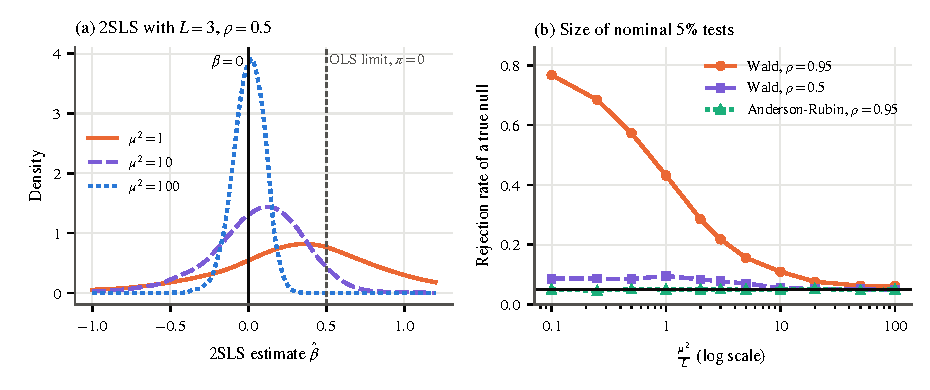
\includegraphics[width=\textwidth]{figures/appA/weakiv.pdf}
\caption{Weak instruments in a simulated design. The model is $y = x\beta + e$, $x = Z\pi + v$ with $\beta = 0$,
$n = 500$, three fixed standard normal instruments, and $(e_i, v_i)$ bivariate normal with unit variances and
correlation $\rho$. The vector $\pi$ is scaled to hit each concentration parameter $\mu^2$ exactly. (a) Kernel
densities of 2SLS over 10,000 replications for $\mu^2 \in \{1, 10, 100\}$ with $\rho = 0.5$. The dashed line marks
$\rho = 0.5$, the OLS limit with irrelevant instruments. (b) Rejection rates of nominal 5 percent tests of the
true null $\beta = 0$, plotted against $\frac{\mu^2}{L}$ on a log scale. The Wald test uses homoskedastic 2SLS
standard errors with $\rho = 0.95$ and $\rho = 0.5$, and the Anderson-Rubin test uses $\rho = 0.95$. The horizontal line is
the nominal size. The Monte Carlo standard error of a rejection rate of 0.05 is 0.0022. Seed 20261022, script
\texttt{sim\_iv.py}.}
\label{fig:A-weakiv}
\end{figure}

\casehead{Diagnostics}
The standard diagnostic is the first-stage $F$ statistic for the excluded instruments.
\citet{StaigerStock1997} suggest treating $F < 10$ as a sign of weak instruments, which by
\cref{prop:A-weak-bias} corresponds to a relative bias of roughly 10 percent. \citet{StockYogo2005} tabulate
cutoffs for the Cragg-Donald version of the statistic under homoskedasticity, for chosen tolerances on
the relative bias of 2SLS or on the size of Wald tests. With heteroskedastic, serially correlated or
clustered errors, the homoskedastic $F$ is invalid. Practitioners then report the robust Wald statistic of
\citet{KleibergenPaap2006}, divided by $L$, and compare it informally with the Stock-Yogo values.
\citet{MontielOleaPflueger2013} derive an \emph{effective} $F$ statistic with valid cutoffs for one
endogenous regressor. With several endogenous regressors, every first-stage $F$ can be large while the
instruments still fail to separate the regressors from one another. The conditional $F$ statistics of
\citet{SandersonWindmeijer2016} address this case. They are needed in the nested logit regression, where both
price and the log within-nest share are endogenous (\cref{sec:07-nl-estimation}). \Cref{tab:A-weakiv}
summarizes the rules.

\begin{table}[htbp]
\centering
\caption{Weak-instrument diagnostics and conventional thresholds}
\label{tab:A-weakiv}
\footnotesize
\begin{tabularx}{\textwidth}{@{}>{\raggedright\arraybackslash}p{0.2\textwidth}
>{\raggedright\arraybackslash}X >{\raggedright\arraybackslash}X >{\raggedright\arraybackslash}p{0.17\textwidth}@{}}
\toprule
Diagnostic & Setting & Threshold & Source \\
\midrule
First-stage $F$ on excluded instruments & One endogenous regressor, homoskedastic errors & $F > 10$ as a rule of
thumb & \citet{StaigerStock1997} \\
\addlinespace
Cragg-Donald $F$ with tabulated cutoffs & Homoskedastic errors, one or more endogenous regressors &
With one endogenous regressor, 9.08 for relative bias of at most 10 percent when $L = 3$, and 16.38
($L = 1$) or 22.30 ($L = 3$) for a nominal 5 percent Wald test with true size of at most 10 percent &
\citet[Tables~5.1--5.2]{StockYogo2005} \\
\addlinespace
Kleibergen-Paap Wald $F$ & Heteroskedastic or clustered errors & No formal cutoffs, compared informally with
the Stock-Yogo values & \citet{KleibergenPaap2006} \\
\addlinespace
Effective $F$ & One endogenous regressor with heteroskedastic, serially correlated or clustered errors & 23.1
as a conservative rule for a 2SLS Nagar bias of at most 10 percent of a worst-case benchmark, at the 5 percent
level & \citet[p.~358]{MontielOleaPflueger2013} \\
\addlinespace
Conditional $F$ & Several endogenous regressors & With $K = 2$, each statistic compared with the Stock-Yogo values
for one endogenous regressor and $L - 1$ instruments & \citet[Section~4]{SandersonWindmeijer2016} \\
\addlinespace
$tF$ adjustment & Just identified, one endogenous regressor & $F > 104.7$ for the usual cutoff of 1.96 to give a
true 5 percent test & \citet{LeeEtAl2022} \\
\bottomrule
\end{tabularx}

\smallskip
\begin{minipage}{0.92\textwidth}\footnotesize
Notes: $L$ is the number of excluded instruments and $K$ the number of endogenous regressors. The cutoffs
depend on the number of instruments and on the chosen tolerance, and the cited sources give full tables.
\end{minipage}
\end{table}

The first-stage $R^2$ is not a weak-instrument diagnostic, because it includes the explanatory power of the
exogenous regressors. \citet[WP fn.~23]{ChaudhuriGoldbergJia2006} report first-stage $R^2$ between 0.57 and 0.95
for their product-group prices, and 0.17 for domestic ciprofloxacin. Their instrument list includes
region-by-product dummies (WP p.~20), which can explain much of the variation in price levels on their own. What
matters is the contribution of the excluded instruments, measured by the partial $R^2$ or the partial $F$
statistic after the exogenous regressors are partialled out. An overall $F$ can also hide weak subsets. In
the simulated markets of \cref{app:problems}, the cluster-robust first-stage $F$ for seven excluded instruments
is 92.5, but six of them are jointly weak with $F = 2.32$. Nearly all the strength comes from one cost shifter.

\casehead{Inference that is robust to weak instruments}
The \emph{Anderson-Rubin test} \citep{AndersonRubin1949} remains valid however weak the instruments are. To test
$H_0\colon\beta = \beta_0$, form $\tilde y = y - x\beta_0$, which equals $e$ under the null. Regress $\tilde y$ on $Z$
and test that all coefficients are zero:
\begin{equation}\label{eq:A-ar}
AR(\beta_0) = \frac{\frac{1}{L}\tilde y^\top P_Z\tilde y}{\frac{1}{n - L}\tilde y^\top M_Z\tilde y} .
\end{equation}
Suppose the errors are normal, homoskedastic and independent of $Z$. Under $H_0$,
$\frac{1}{\sigma_e^2}e^\top P_Ze \sim \chi^2_L$ and $\frac{1}{\sigma_e^2}e^\top M_Ze \sim \chi^2_{n - L}$, because $P_Z$ and
$M_Z$ are idempotent with ranks $L$ and $n - L$. The two quadratic forms are independent because $P_ZM_Z = 0$.
Hence $AR(\beta_0) \sim F(L, n - L)$ exactly, whatever the value of $\pi$. With $K_1$ exogenous regressors partialled
out, the denominator degrees of freedom become $n - L - K_1$. Without normality, $L \cdot AR(\beta_0)$ is
asymptotically $\chi^2_L$, and heteroskedasticity- or cluster-robust versions use a robust Wald test of the
coefficients on $Z$.

A confidence set collects the values $\beta_0$ that the test does not reject. The Anderson-Rubin set can be a
bounded interval, the union of two rays, the whole real line, or even empty. An unbounded set is the right
answer when the data carry little information about $\beta$. In panel (b) of \cref{fig:A-weakiv}, the
Anderson-Rubin test rejects between 4.7 and 5.3 percent of the time at every instrument strength. Its
weakness is power when $L > K$, because it tests $\beta = \beta_0$ jointly with the overidentifying restrictions.
The conditional likelihood ratio test of \citet{Moreira2003} is more powerful, and it coincides with the
Anderson-Rubin test in the just-identified case. \citet{AndrewsStockSun2019} survey these methods.

\casehead{Many instruments}
Adding instruments that carry little information raises $L$ without raising $\mu^2$, and by
\cref{prop:A-weak-bias} it pushes 2SLS toward OLS. In the limit with as many instruments as observations,
$P_Z = I_n$ and 2SLS equals OLS. Limited-information maximum likelihood (LIML) is approximately median-unbiased
and much less sensitive to the number of instruments. The jackknife IV estimator removes the own-observation
term that causes the bias \citep{AngristImbensKrueger1999}. In demand estimation, \citet{Armstrong2016} shows
that the characteristics of rival products can be weak instruments in markets with many products. Markups then
converge to limits that hardly depend on rivals' characteristics (\cref{sec:08-iv-families}).

\subsection{Specification tests}\label{sec:A-spectests}

\casehead{Overidentification}
When $L > K$, the instruments imply more moment conditions than parameters, and we can test whether they are
mutually consistent. Under homoskedasticity, the \emph{Sargan statistic} is $n$ times the $R^2$ of the
regression of the 2SLS residuals on all instruments. It converges to $\chi^2_{L - K}$ under the null that every
instrument is exogenous \citep{Sargan1958}. Hansen's $J$ statistic is the robust version
(\cref{thm:A-jtest}). \citet[pp.~23--24]{Dafny2005} splits her instrument into the number of rival pairs less than
0.2 miles apart and the number between 0.2 and 0.3 miles apart. The Sargan statistic is 0.36 with a $p$-value
of 0.55, so the two bands imply similar effects. The test has limits. It is identically zero in a
just-identified model. It has no power against a bias that all instruments share. Both of Dafny's bands
measure distances between the same hospitals, so they would fail together if co-location itself were
correlated with unobserved price growth.

\casehead{The Hausman principle}
A second family of tests compares two estimators. One is efficient under the null hypothesis, and the other
is consistent under both the null and the alternative.

\begin{lemma}[Hausman]\label{lem:A-hausman}
Let $\hat\beta_E$ and $\hat\beta_C$ be estimators of $\beta$ such that, under $H_0$,
$\sqrt{n}\bigl((\hat\beta_E - \beta)^\top, (\hat\beta_C - \beta)^\top\bigr)^\top$ converges to a normal vector with
variances $V_E$ and $V_C$ and cross-covariance $C = \mathrm{Acov}(\hat\beta_E, \hat\beta_C)$. Here $\mathrm{Avar}$
and $\mathrm{Acov}$ denote the asymptotic variance and covariance of $\sqrt{n}$ times the centered estimators. If $\hat\beta_E$ is
asymptotically efficient under $H_0$, then $C = V_E$. Equivalently, $\hat\beta_E$ is asymptotically uncorrelated
with $\hat\beta_C - \hat\beta_E$, and
\begin{equation}\label{eq:A-hausman-var}
\mathrm{Avar}(\hat\beta_C - \hat\beta_E) = V_C - V_E .
\end{equation}
\end{lemma}

\begin{proof}
Write $D = \hat\beta_C - \hat\beta_E$, which converges to zero under $H_0$. Its asymptotic covariance with
$\hat\beta_E$ is $C - V_E$. For fixed vectors $a$ and $b$ and a scalar $\lambda$, the estimator
$a^\top\hat\beta_E + \lambda b^\top D$ is consistent for $a^\top\beta$. Its asymptotic variance is
\begin{equation*}
f(\lambda) = a^\top V_Ea + 2\lambda\,a^\top(C - V_E)b + \lambda^2\,b^\top\mathrm{Avar}(D)\,b .
\end{equation*}
Efficiency of $\hat\beta_E$ requires $f(\lambda) \ge f(0)$ for every $\lambda$, so the derivative at zero,
$2a^\top(C - V_E)b$, must vanish. This holds for all $a$ and $b$, so $C = V_E$. Then
$\mathrm{Avar}(D) = V_C - C - C^\top + V_E = V_C - V_E$.
\end{proof}

The \emph{Hausman statistic} is
\begin{equation}\label{eq:A-hausman}
\mathcal{H} = (\hat\beta_C - \hat\beta_E)^\top\bigl[\hat V_C - \hat V_E\bigr]^{-}(\hat\beta_C - \hat\beta_E)
\xrightarrow{d} \chi^2_q ,
\end{equation}
where $\hat V_C$ and $\hat V_E$ estimate the finite-sample variances, the superscript denotes a generalized
inverse, and $q$ is the rank of $V_C - V_E$ \citep{Hausman1978}. When OLS is compared with 2SLS, $q$ equals the
number of endogenous regressors tested. Two practical problems arise. The estimated difference
$\hat V_C - \hat V_E$ need not be positive semidefinite in finite samples, and OLS is efficient only under
homoskedasticity. The regression form avoids both. Add the first-stage residuals of the suspect regressors to
the OLS regression, as in \cref{prop:A-cf-2sls}, and test that their coefficients are jointly zero with a
robust Wald test. Under homoskedasticity this test is asymptotically equivalent to \eqref{eq:A-hausman}.

The principle appears throughout the book.
\begin{itemize}
\item \citet{Borenstein1989} rejects exogeneity of the route share and the route Herfindahl index, and so
  reports 2SLS. A Hausman test does not reject exogeneity of the load factor ``at any reasonable significance
  level'', so he treats it as exogenous (pp.~352 and 356--357). The cost of instrumenting shows in his Table 2.
  For the 80th percentile fare, the route-share coefficient is 0.1259 (0.0349) by OLS and 0.2238 (0.0784) by
  2SLS. The route Herfindahl coefficient moves from $-0.0120$ (0.0425) to $-0.1787$ (0.0901). The 2SLS standard
  errors are more than twice the OLS ones.
\item \citet[p.~21]{Dafny2005} reports that Hausman tests easily reject equality of the IV and OLS estimates
  in \cref{tab:A-dafny}.
\item \citet{Hausman1997} notes that weekly supermarket prices may be predetermined with respect to demand
  shocks, in which case OLS is consistent and efficient. A Hausman test of OLS against IV can decide
  (\cref{sec:10-hausman-identification}).
\item In panel data, random effects is efficient under its assumptions and fixed effects is consistent
  whether or not the unit effects are correlated with the regressors. Their difference tests
  $\E[\alpha_i \mid x_{i1}, \dots, x_{iT}] = 0$ (\cref{sec:A-panel}).
\item The test of independence of irrelevant alternatives of \citet{HausmanMcFadden1984} compares logit
  estimates from the full choice set with estimates from a restricted set. The restricted estimates are
  consistent under both hypotheses and inefficient under the null (\cref{eq:10-hm-test}).
\end{itemize}

\subsection{What IV estimates when effects differ}\label{sec:A-late}

So far the effect of $x_i$ has been the same for every unit. When effects differ, IV estimates a weighted
average of them, and the weights depend on the instrument.

\begin{theorem}[Local average treatment effect]\label{thm:A-late}
Let $z_i$ and $d_i$ be binary. Each unit has potential treatments $d_i(1)$ and $d_i(0)$, one for each value of
the instrument, and potential outcomes $y_i(d, z)$. Assume the following.
\begin{enumerate}[label=(\roman*)]
\item The instrument is independent of the potential outcomes and treatments
  $\{y_i(d, z), d_i(z) : d, z \in \{0, 1\}\}$.
\item The instrument is excluded from the outcome, $y_i(d, 1) = y_i(d, 0) \equiv y_i(d)$ for $d = 0, 1$.
\item The instrument is relevant, $\E[d_i(1) - d_i(0)] \neq 0$.
\item Treatment is monotone in the instrument, $d_i(1) \ge d_i(0)$ for every $i$.
\end{enumerate}
Then the Wald estimand \eqref{eq:A-wald-estimator} equals
$\E[y_i(1) - y_i(0) \mid d_i(1) > d_i(0)]$, the average effect for \emph{compliers}, the units whose treatment
the instrument changes \citep{ImbensAngrist1994}.
\end{theorem}

\begin{proof}
By exclusion, the observed outcome is $y_i = y_i(0) + d_i(z_i)\bigl(y_i(1) - y_i(0)\bigr)$. By independence,
\begin{equation*}
\E[y_i \mid z_i = 1] - \E[y_i \mid z_i = 0] = \E\bigl[\bigl(d_i(1) - d_i(0)\bigr)\bigl(y_i(1) - y_i(0)\bigr)\bigr] .
\end{equation*}
Monotonicity makes $d_i(1) - d_i(0)$ equal to one for compliers and zero for everyone else, so the right side
equals $\Pr(\text{complier})\,\E[y_i(1) - y_i(0) \mid \text{complier}]$. Independence also gives
$\E[d_i \mid z_i = 1] - \E[d_i \mid z_i = 0] = \E[d_i(1) - d_i(0)] = \Pr(\text{complier})$, which is nonzero by
relevance. The ratio is the complier average effect.
\end{proof}

The population splits into \emph{always-takers} ($d_i(1) = d_i(0) = 1$), \emph{never-takers}
($d_i(1) = d_i(0) = 0$), compliers, and \emph{defiers} ($d_i(1) < d_i(0)$), whom monotonicity rules out.
Different instruments move different compliers, so two valid instruments can identify different averages, and
an overidentification test can then reject even though both instruments are exogenous. With a continuous
endogenous variable, \citet{AngristGraddyImbens2000} show that the linear IV estimand in a supply and demand
system is a weighted average of the derivatives of the structural function. The weights are largest at
prices where the instrument shifts the equilibrium most. Dafny's estimate is local in this sense, since the
instrument moves only mergers of co-located hospitals.

\casehead{An IO analogue}
\citet{Corts1999} makes the same point about conduct. Write the supply relation as $P_t - c_t = \theta_tm_t$, with
conduct $\theta_t$ and $m_t = Q_t\bigl\lvert\frac{\partial Q_t}{\partial P_t}\bigr\rvert^{-1}$. Suppose marginal cost is known and a
demand shifter $Z_t$ serves as the instrument for $m_t$ in an equation with a constant conduct parameter. The
IV estimand is
\begin{equation*}
\frac{\Cov(Z_t, P_t - c_t)}{\Cov(Z_t, m_t)} = \frac{\Cov(Z_t, \theta_tm_t)}{\Cov(Z_t, m_t)} ,
\end{equation*}
which for small demand movements is approximately $\frac{\dd(\theta m)}{\dd m} = \theta + m\frac{\dd\theta}{\dd m}$.
The estimator recovers the marginal response of the markup to demand, which can differ sharply from the average
level of conduct. If $\theta_t = a - b\,m_t$, then $\theta_tm_t = am_t - bm_t^2$ and the estimand is
$a - b\frac{\Cov(Z_t, m_t^2)}{\Cov(Z_t, m_t)}$. With $\bar m = \E[m_t]$,
\begin{equation*}
\Cov(Z_t, m_t^2) = 2\bar m\Cov(Z_t, m_t) + \E\bigl[(Z_t - \E Z_t)(m_t - \bar m)^2\bigr] .
\end{equation*}
When the last term is zero, for example when $(Z_t, m_t)$ is jointly symmetric about its mean, the estimand is
$a - 2b\bar m$, while average conduct is $a - b\bar m$ (\cref{sec:03-corts}). Otherwise the third-moment term moves the
estimand away from $a - 2b\bar m$. In both cases the estimand can lie outside the range of $\theta_t$.

\subsection{System IV: three-stage least squares}\label{sec:A-3sls}

When several equations each contain endogenous regressors, they can be estimated jointly. Stack $G$ equations
$y_g = X_g\beta_g + e_g$ with a common $n \times L$ instrument matrix $Z$, block-diagonal $X$, and error vector
$e_t = (e_{1t}, \dots, e_{Gt})^\top$ with $\E[e_te_t^\top \mid z_t] = \Sigma$. The moment conditions are
$\E[e_t \otimes z_t] = 0$, and under conditional homoskedasticity their covariance matrix is
$\E[(e_t \otimes z_t)(e_t \otimes z_t)^\top] = \Sigma \otimes \E[z_tz_t^\top]$. Efficient GMM (\cref{sec:A-gmm-efficient}) weights the
sample moments $(I_G \otimes Z^\top)(y - X\beta)$ by the inverse of this matrix, estimated by
$\hat\Sigma^{-1} \otimes (Z^\top Z)^{-1}$. Since
$(I_G \otimes Z)(\hat\Sigma^{-1} \otimes (Z^\top Z)^{-1})(I_G \otimes Z^\top) = \hat\Sigma^{-1} \otimes P_Z$, the first-order
condition gives the \emph{three-stage least squares} (3SLS) estimator of \citet{ZellnerTheil1962},
\begin{equation}\label{eq:A-3sls}
\hat\beta_{3SLS} = \bigl[X^\top(\hat\Sigma^{-1} \otimes P_Z)X\bigr]^{-1}X^\top(\hat\Sigma^{-1} \otimes P_Z)\,y .
\end{equation}
The three stages are the first-stage regressions, 2SLS for each equation to estimate
$\hat\Sigma_{gh} = \frac{1}{n}\hat e_g^\top\hat e_h$, and the system estimator \eqref{eq:A-3sls}. By the logic of
\cref{prop:A-sur-ols}, 3SLS equals equation-by-equation 2SLS when $\Sigma$ is diagonal or every equation is
exactly identified. Its gains come from correlated errors and from restrictions across equations. Its cost is
that misspecification of any one equation contaminates the estimates of all of them. The estimated $\Sigma$
also adds noise in small samples.

\casehead{Application: residual demand in brewing}
\citet{BakerBresnahan1988} estimate the inverse residual demand curves of Anheuser-Busch, Pabst and Coors
jointly by 3SLS. Each equation regresses the firm's log price on its log quantity, demand shifters and cost
variables. The coefficient on own quantity, $\eta^R_j$, is the inverse elasticity of residual demand. Own
quantity is instrumented by firm-specific cost shifters: capacity for every firm, average plant size for
Anheuser-Busch and Pabst, and the Colorado manufacturing wage for Coors, which brewed only in Golden. The joint
estimation exploits the correlation of errors across the three equations. It also imposes a cross-equation
restriction, under which industry cost variables enter every equation through one common marginal cost index
(their eq.~12). The data are annual for 1962--1982, so each equation has only 21 observations (Table 3).

The estimates of $\eta^R_j$ are $-0.745$ (0.054) for Coors, $-0.058$ (0.031) for Pabst and $-0.312$ (0.064) for
Anheuser-Busch before 1975. An interaction with the post-1975 period, when light beer was introduced, is 0.282
(0.040), so Anheuser-Busch's inverse elasticity falls to $-0.030$ after 1975 (Table 3). Single-equation 2SLS gives
similar elasticities ``with little noticeable efficiency loss'' (fn.~20). Treating quantity as exogenous gives
$-0.738$, $-0.053$ and $-0.312$ (fn.~26), so simultaneity bias is small in these data. With 21 observations per
equation, several regressors and an estimated three-by-three covariance matrix, the asymptotic standard errors
should be read with caution. \Cref{sec:03-residual-demand} interprets the results.

The estimators of this section all have closed forms. Many structural models in industrial organization do not.
Their parameters enter nonlinearly, their errors enter through an equilibrium, or their likelihood involves an
integral. \Cref{sec:A-extremum} therefore turns to estimators defined by optimizing a criterion, which include
2SLS and 3SLS as special cases, and \cref{sec:A-twostep} returns to the joint estimation of demand and supply.
